\documentclass[12pt]{article}
\usepackage[utf8]{inputenc}
\usepackage[T1]{fontenc}
\usepackage{amsmath}
\usepackage{amsfonts}
\usepackage{amssymb}
\usepackage[version=4]{mhchem}
\usepackage{stmaryrd}
\usepackage{hyperref}
\hypersetup{colorlinks=true, linkcolor=blue, filecolor=magenta, urlcolor=cyan}
\urlstyle{same}
\usepackage{caption}
\usepackage{graphicx}
\usepackage[export]{adjustbox}
\graphicspath{ {./figures/} }
\usepackage{bbold}
\usepackage[margin=1in]{geometry}

\title{Practicing Dynare: \\ A Fiscal Policy Focus}

\author{\\%Contributors: Hylton Hollander, Clinton Joel, Julius Pain
}
\date{01 December 2025 \\ Work-in-Progress \\ \sc{Not for Distribution}}
% December 4, 2010


\usepackage{listings}
\lstset{basicstyle=\ttfamily\footnotesize,breaklines=true,columns=fullflexible,keepspaces=true}
\begin{document}
\maketitle
%\captionsetup{singlelinecheck=false}

% \footnotetext{*We thank Michele Juillard for helpful comments on an earlier draft.\\ ${ }^{\dagger}$ Authors’ emails: Barillas: \href{mailto:fvb201@nyu.edu}{fvb201@nyu.edu}, Bhandari: \href{mailto:apb296@nyu.edu}{apb296@nyu.edu}, Colacito: \href{mailto:riccardo.colacito@unc.edu}{riccardo.colacito@unc.edu}, Kitao: \href{mailto:sk910@nyu.edu}{sk910@nyu.edu}, Matthes, \href{mailto:cm1518@nyu.edu}{cm1518@nyu.edu}, Sargent: \href{mailto:ts43@nyu.edu}{ts43@nyu.edu}, Shin: \href{mailto:yshin@wustl.edu}{yshin@wustl.edu}. }

\begin{abstract}
%This note builds on ``Practicing Dynare'' by Barillas et al. (2010). It teaches Dynare by applying it to nine dynamic stochastic general equilibrium models with a fiscal policy focus. We hope it illustrates the efficacy of learning by doing.
\noindent This document updates the \textit{Practicing Dynare} document and codebase by Barillas et al. (2010) and provides a structured path for learning how to implement and analyse fiscal policy in RBC and DSGE models using Dynare (Version 6 as of 2025). The goal is to move from simple stochastic growth models to fully deterministic fiscal transition experiments as presented in Chapter 11 of Ljungqvist \& Sargent (2012). Each example is designed to be minimal, transparent, and directly linked to the corresponding Dynare \texttt{.mod} file. The document emphasises hands-on learning: running code, inspecting steady states, and interpreting transition dynamics. By the end, users should be comfortable modifying the fiscal instruments, creating their own policy scenarios, and understanding how fiscal shocks propagate through standard macroeconomic environments. Section 6 reserves space for the flexible-price NT-DSGE model, which is maintained separately and is not implemented by the examples in this repository.
\end{abstract}

\pagebreak

\tableofcontents

\pagebreak

\section{Introduction}
Sections 2 and 3 solve and estimate stochastic growth models. Sections 4 and 5 implement deterministic fiscal experiments, including anticipated changes and elastic labour supply. Section 6 remains a placeholder for the separate NT-DSGE model. The runnable files are in \texttt{Code/sections}; original 2025 revisions are preserved separately. Historical figures, tables, posterior summaries and figure-number mappings have not yet been revalidated. All anticipated changes at text date $t=10$ occur in simulation period 11, since simulation period 1 denotes $t=0$. Investment instrument $\tau_i$ denotes a subsidy, with purchase price $1-\tau_i$. Prices $q_t$ are dated Arrow--Debreu prices; they should not be added as an unnormalised recursive state with an arbitrary steady-state level.

%Some of our examples bear eloquent witness to the technological improvements brought by Dynare. For example, the maximum likelihood estimates in Sargent (1977) and Hansen, Sargent, and Tallarini (1999) were time-consuming and painful to obtain originally. Dynare has reduced the time and the pain.

%Section 6 estimates a rational expectations model of hyperinflation originally formulated by Sargent (1977). Section 7 solves and estimates the permanent income model of Hall (1988). This application is interesting, among other reasons, for the way that it illustrates how Dynare can implement the 'diffuse Kalman filter' needed in situations in which an initial endogenous state variable is unknown and the model has a unit root. Section 8 solves and estimates the Ryoo and Rosen (2004) rational expectations model of a market for engineers. Section 9 estimates a model of consumption growth proposed by Bansal and Yaron (2004). Section 10 solves and estimates the Hansen, Sargent, and Tallarini (1999) model of robust permanent income and pricing. Section 11 solves and estimates the Bansal and Yaron (2004) of asset prices and long-run risk in consumption and dividends. 


The listings below are the short participant examples. Self-contained files in \path{Code/full_replications} produce the corresponding section outputs. Command explanations and the figure-name map are in \path{notes/README.md}. Historical images retain a \texttt{\_legacy} suffix pending the separate replication comparison.

\section{The Neoclassical growth model}
\subsection*{2.1 The model}
We study a widely used stochastic neoclassical growth model with leisure (see, for example, Cooley and Prescott (1995)). A representative household's problem is

$$
\max _{\left\{c_{t}, l_{t}\right\}_{t=0}^{\infty}} E_{0} \sum_{t=1}^{\infty} \beta^{t-1} \frac{\left(c_{t}^{\theta}\left(1-l_{t}\right)^{1-\theta}\right)^{1-\tau}}{1-\tau}
$$

subject to the resource constraint


\begin{equation*}
c_{t}+i_{t}=e^{z_{t}} k_{t}^{\alpha} l_{t}^{1-\alpha} \tag{1}
\end{equation*}


the law of motion for capital


\begin{equation*}
k_{t+1}=i_{t}+(1-\delta) k_{t} \tag{2}
\end{equation*}


and the stochastic process for productivity


\begin{equation*}
z_{t}=\rho z_{t-1}+s \epsilon_{t} \tag{3}
\end{equation*}


with $\epsilon_{t} \sim N\left(0, \sigma^{2}\right)$.\\
The system of equations characterizing an equilibrium is comprised of equations (1), (2) and (3), the Euler intertemporal condition


\begin{equation*}
\frac{\left(c_{t}^{\theta}\left(1-l_{t}\right)^{1-\theta}\right)^{1-\tau}}{c_{t}}=\beta E_{t}\left[\frac{\left(c_{t+1}^{\theta}\left(1-l_{t+1}\right)^{1-\theta}\right)^{1-\tau}}{c_{t+1}}\left(1+\alpha e^{z_{t+1}} k_{t+1}^{\alpha-1} l_{t+1}^{1-\alpha}-\delta\right)\right] \tag{4}
\end{equation*}


and an optimality condition for supply of labor


\begin{equation*}
\frac{1-\theta}{\theta} \frac{c_{t}}{1-l_{t}}=(1-\alpha) e^{z_{t}} k_{t}^{\alpha} l_{t}^{-\alpha} . \tag{5}
\end{equation*}


Use (1) and (2) to get


\begin{equation*}
k_{t+1}=e^{z_{t}} k_{t}^{\alpha} l_{t}^{1-\alpha}-c_{t}+(1-\delta) k_{t} . \tag{6}
\end{equation*}


An equilibrium is characterized by a system of four equations (3), (4), (5) and (6).

\subsection*{2.2 Calibration and approximation}
\subsection*{2.2.1 Calibration}
To estimate the policy function, parameters that enter the model are calibrated as in Table 1. For more on the calibrations of the related parameters, please see, for example, Cooley and Prescott (1995).

\subsection*{2.2.2 Approximation}
The following file implements the model in Dynare. The stochastic Euler equation uses next-period marginal product, consistent with equations (1)--(6).

\lstinputlisting{Code/sections/s02_02_growth_approx.mod}

\begin{figure}[!htbp]
\begin{center}
  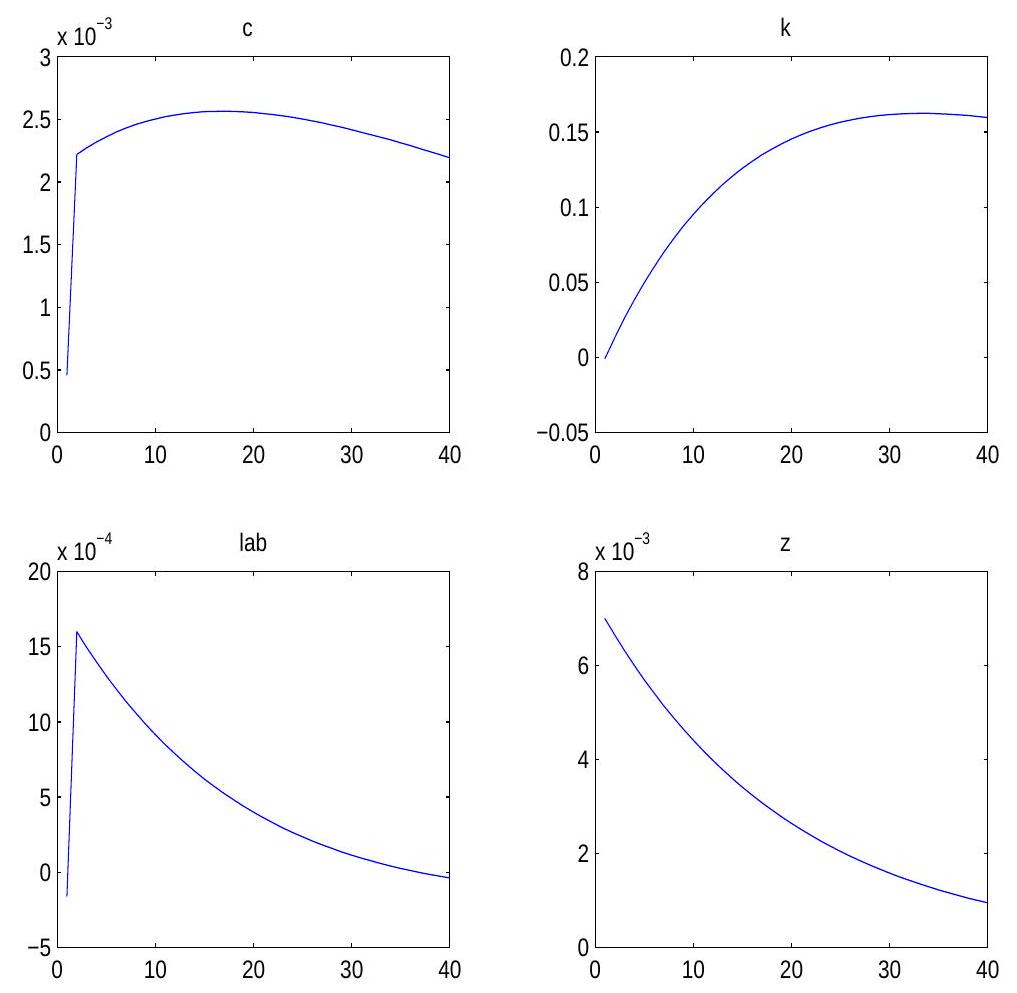
\includegraphics[width=\textwidth]{s02_02_growth_irfs_legacy.jpg}
\captionsetup{labelformat=empty}
\caption{Figure 1: Impulse response function to a technology shock}
\end{center}
\label{fig:s02-02-growth-irfs-legacy}
\end{figure}


\begin{table}[h]
\begin{center}
\begin{tabular}{cc}
\hline\hline
Parameter & Calibration \\
\hline
$\beta$ & 0.987 \\
$\theta$ & 0.357 \\
$\delta$ & 0.012 \\
$\alpha$ & 0.4 \\
$\tau$ & 2 \\
$\rho$ & 0.95 \\
$s$ & 0.007 \\
$\sigma$ & 1 \\
\hline\hline
\end{tabular}
\captionsetup{labelformat=empty}
\caption{Table 1: Parameters' calibration}
\end{center}
\end{table}

The historical Table 2 reports the coefficients of the approximated policy functions and transition functions.

\begin{table}[h]
\begin{center}
\begin{tabular}{|l|l|l|l|l|}
\hline
 & k & z & c & lab \\
\hline
Constant & 54.615371 & 0 & 0.960775 & 0.543716 \\
\hline
k (-1) & 0.983153 & 0 & 0.011727 & -0.001668 \\
\hline
z (-1) & 1.978406 & 0.950000 & 0.317480 & 0.228716 \\
\hline
e & -0.000935 & 0.007000 & 0.000454 & -0.000162 \\
\hline
k (-1),k (-1) & -0.000038 & 0 & -0.000030 & 0.000011 \\
\hline
$\mathrm{z}(-1), \mathrm{k}(-1)$ & 0.011128 & 0 & 0.002996 & 0.000762 \\
\hline
$\mathrm{z}(-1), \mathrm{z}(-1)$ & 1.253721 & 0 & 0.096224 & -0.046394 \\
\hline
e,e & -0.000003 & 0 & 0.000001 & 0 \\
\hline
k (-1),e & -0.000002 & 0 & 0.000002 & 0.000001 \\
\hline
z (-1),e & -0.001076 & 0 & 0.000430 & -0.000056 \\
\hline
\end{tabular}
\captionsetup{labelformat=empty}
\caption{Table 2: Policy and transition functions.}
\end{center}
\end{table}


\subsection*{2.3 Estimation}
The simulated data series for consumption are used to estimate some unknown parameters of the model. Suppose we would like to estimate the preference parameters $\theta$ and $\tau$, and the stochastic process for productivity, summarized by two parameters $\rho$ and $\sigma$. The following code instructs Dynare to conduct the estimation.

\lstinputlisting{Code/sections/s02_03_growth_estimate.mod}

\begin{figure}[!htbp]
\begin{center}
  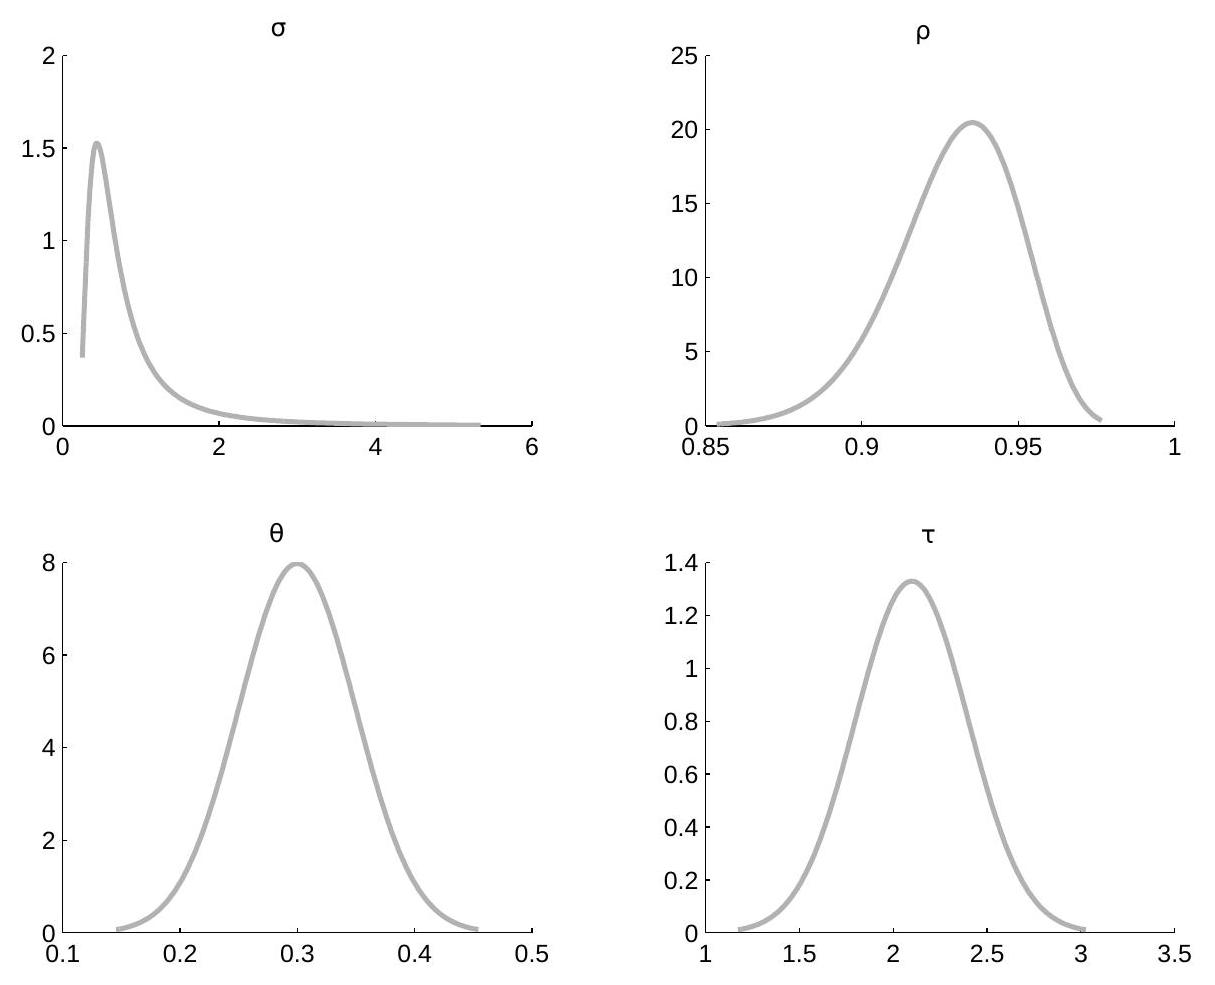
\includegraphics[width=\textwidth]{s02_03_priors_legacy.jpg}
\captionsetup{labelformat=empty}
\caption{Figure 2: Priors.}
\end{center}
\label{fig:s02-03-priors-legacy}
\end{figure}

\begin{figure}[!htbp]
\begin{center}
  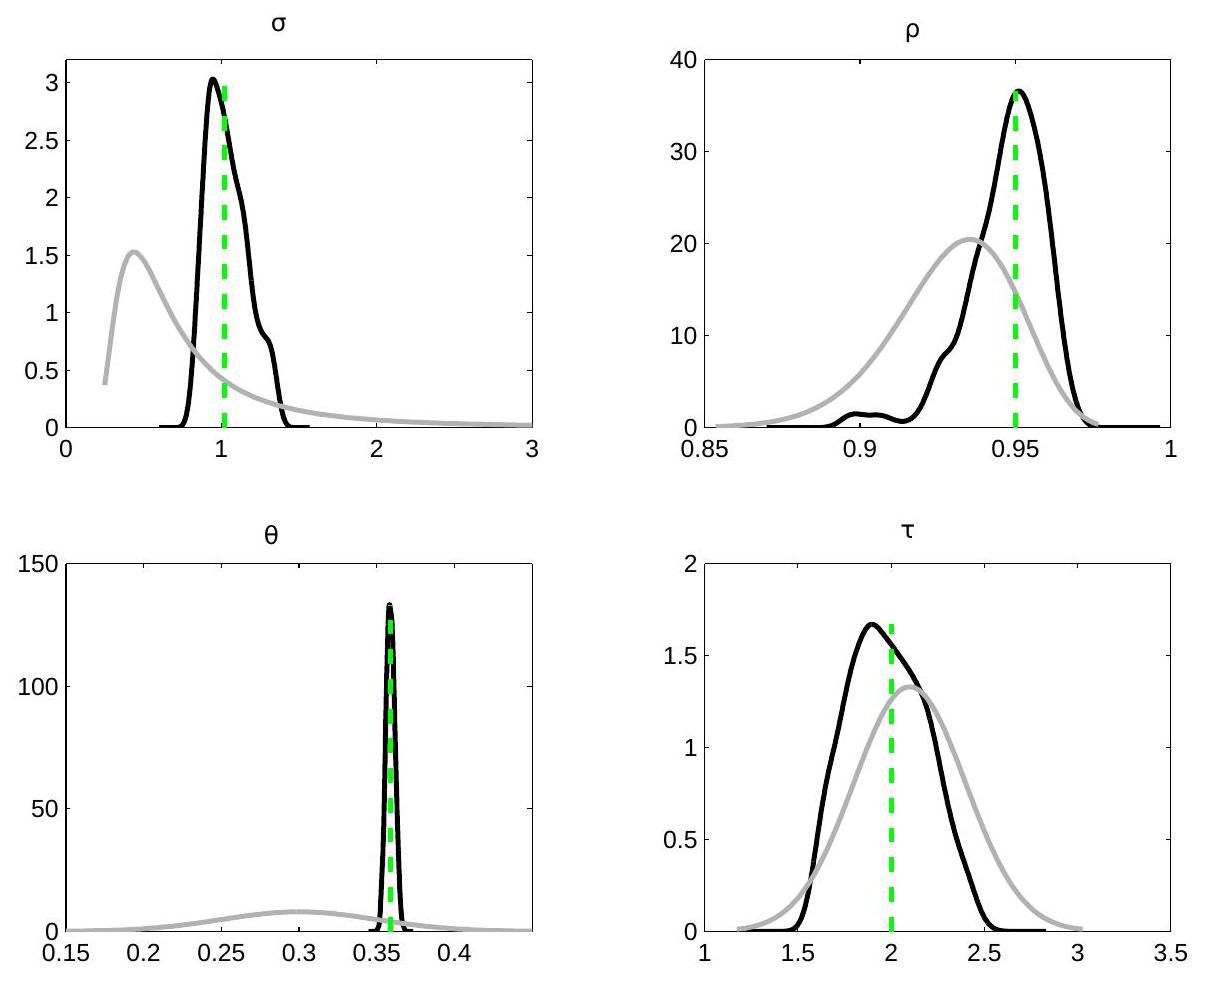
\includegraphics[width=\textwidth]{s02_03_posterior_legacy.jpg}
\captionsetup{labelformat=empty}
\caption{Figure 3: Posterior.}
\end{center}
\label{fig:s02-03-posterior-legacy}
\end{figure}


Table 3 records the historical priors. The runnable example uses a beta prior for the consumption share and a finite-spread innovation standard-deviation prior (mean 1, standard deviation 0.2). These changes impose economic bounds and regularise a short teaching run. Table 4 is historical output and is not a result of the revised estimation file.


\begin{table}[!htbp]
\begin{center}
\begin{tabular}{cccc}
\hline\hline
Parameter & Distribution & Mean & Std.Dev. \\
\hline
$\rho$ & Beta & 0.93 & 0.02 \\
$\theta$ & Normal & 0.3 & 0.05 \\
$\tau$ & Normal & 2.1 & 0.3 \\
$\sigma$ & Inv. Gamma & 0.95 & inf. \\
\hline\hline
\end{tabular}
\captionsetup{labelformat=empty}
\caption{Table 3: Priors}
\end{center}
\end{table}

\begin{table}[h]
\begin{center}
\captionsetup{labelformat=empty}
\caption{Table 4: Historical posterior (not revalidated)}
\begin{tabular}{lcccccc}
\hline\hline
 & prior mean & post. mean & conf. & interval & prior dist & prior std \\
\hline
$\rho$ & 0.930 & 0.9480 & 0.9319 & 0.9645 & beta & 0.0200 \\
$\theta$ & 0.300 & 0.3589 & 0.3540 & 0.3645 & norm & 0.0500 \\
$\tau$ & 2.100 & 2.0046 & 1.6532 & 2.3356 & norm & 0.3000 \\
$\sigma$ & 0.950 & 1.0227 & 0.8321 & 1.2175 & invg & Inf \\
\hline\hline
\end{tabular}
\end{center}
\end{table}


\section{International Business Cycle Model}
We study a simplified version of the two-country production model in Kim and Kim (2003).

\subsection*{3.1 The model}
Two countries are identical ex-ante and markets are complete. A solution to a Pareto planner's problem is characterized by the following equations

$$
\begin{aligned}
C_{1, t} & =C_{2, t} \\
C_{1, t}^{-\gamma} & =\beta \mathbb{E}_{t} C_{1, t+1}^{-\gamma}\left(\alpha A_{1, t+1} K_{1, t+1}^{\alpha-1}+1-\delta\right) \\
C_{2, t}^{-\gamma} & =\beta \mathbb{E}_{t} C_{2, t+1}^{-\gamma}\left(\alpha A_{2, t+1} K_{2, t+1}^{\alpha-1}+1-\delta\right) \\
A_{1, t} K_{1, t}^{\alpha}+A_{2, t} K_{2, t}^{\alpha} & =C_{1, t}+C_{2, t}+K_{1, t+1}-(1-\delta) K_{1, t}+K_{2, t+1}-(1-\delta) K_{2, t} \\
\ln A_{1, t+1} & =\rho \ln A_{1, t}+\epsilon_{1, t+1} \\
\ln A_{2, t+1} & =\rho \ln A_{2, t}+\epsilon_{2, t+1}
\end{aligned}
$$

The first three equalities are the first-order conditions with regard to the consumption ( $C_{i, t}$ ), and the fourth one is the world resource constraint. The last two describe the law of motion for the technological shock $\left(A_{i, t}\right) . K_{i, t}$ denotes the capital stock of country $i$ at time $t$.

\subsection*{3.2 Calibration and approximation}
\subsection*{3.2.1 Calibration}
The following parameter values are used.

\begin{table}[h]
\begin{center}
\begin{tabular}{cc}
\hline\hline
Parameter & Calibration \\
\hline
$\beta$ & 0.98 \\
$\delta$ & 0.05 \\
$\alpha$ & 0.4 \\
$\rho$ & 0.85 \\
$\sigma_{\epsilon_{1}}$ & 0.08 \\
$\sigma_{\epsilon_{2}}$ & 0.08 \\
\hline\hline
\end{tabular}
\captionsetup{labelformat=empty}
\caption{Table 5: Parameter Values}
\end{center}
\end{table}

Dynare computes the policy function as a second-order approximation around the (log) steady-state. The .mod Dynare file of the system is as follows.

\lstinputlisting{Code/sections/s03_02_twocountry_approx.mod}

\begin{figure}[!htbp]
\begin{center}
  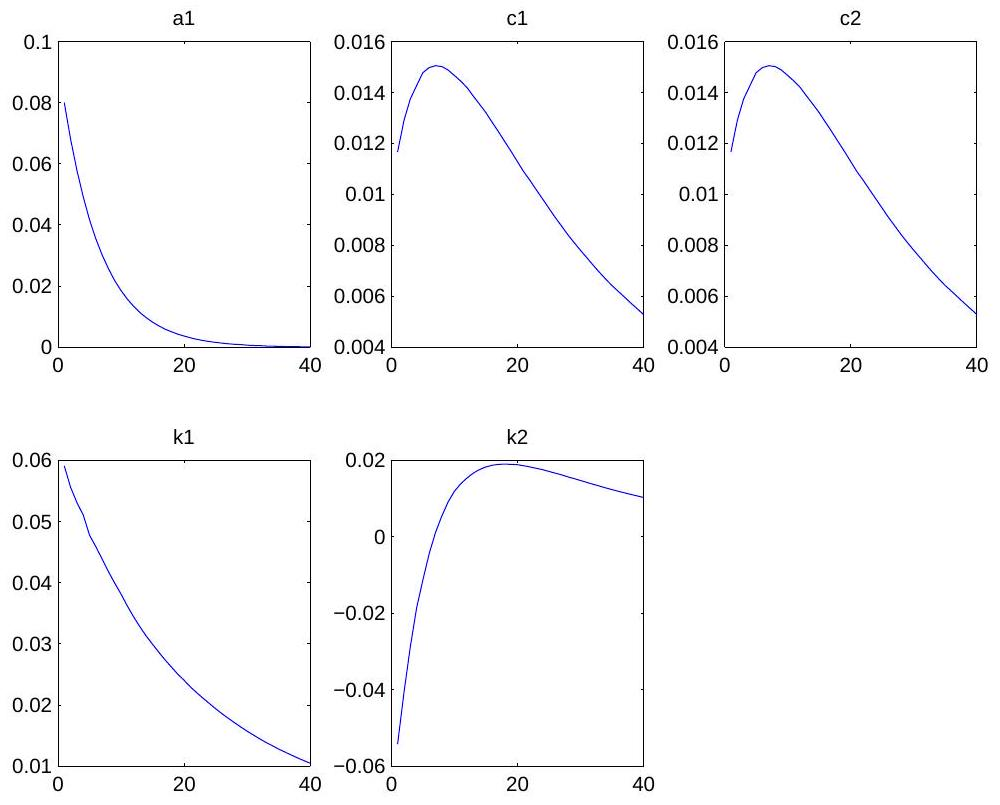
\includegraphics[width=\textwidth]{s03_02_twocountry_irfs_legacy.jpg}
\captionsetup{labelformat=empty}
\caption{Figure 4: Impulse response function $(\epsilon_1)$}
\end{center}
\label{fig:s03-02-twocountry-irfs-legacy}
\end{figure}


The historical output is given as a matrix of coefficients for the policy function; the numerical coefficients below have not been revalidated against the revised code. From this matrix, for example, one can construct the optimal consumption rule for Country 1:

$$
\begin{aligned}
\hat{c}_{1, t}= & 0.824+0.243\left(\hat{k}_{1, t}+\hat{k}_{2, t}\right)+0.140\left(\hat{a}_{1, t}+\hat{a}_{2, t}\right)+0.062\left(\hat{k}_{1, t-1}^{2}+\hat{k}_{2, t-1}^{2}\right)-0.110 \hat{k}_{1, t} \hat{k}_{2, t} \\
& -0.015\left(\hat{a}_{1, t} \hat{k}_{1, t}+\hat{a}_{2, t} \hat{k}_{2, t}\right)-0.032\left(\hat{a}_{1, t} \hat{k}_{2, t}+\hat{a}_{2, t} \hat{k}_{1, t}\right)+0.044\left(\hat{a}_{1, t}^{2}+\hat{a}_{2, t}^{2}\right)-0.040 \hat{a}_{1, t} \hat{a}_{2, t},
\end{aligned}
$$

where $\hat{y}$ denotes the deviation of $\ln Y$ from its log steady-state. Note that Dynare breaks $\hat{a}_{i, t}$ into $\hat{a}_{i, t-1}$ and $\epsilon_{i, t}$, so the output from Dynare looks unnecessarily messy.

Dynare also produces the associated impulse response functions of the system. Figure 4 illustrate the response of the system to a one-standard-deviation shock to $\epsilon_{1}$.

The approximation file saves named observable series in a section-specific MAT file. Run it before the corresponding estimation example. The random seed is fixed for repeatability.

\subsection*{3.3 Estimation}
Now assume that we do not know the true parameter values. We can estimate the unknown parameters from the saved data, using the Bayesian econometrics function of Dynare.

We will estimate 4 parameters $\rho, \alpha, \sigma_{\epsilon_{1}}$, and $\sigma_{\epsilon_{2}}$. Hence, we specify a prior distribution for each parameter. The revised runnable exercise uses beta priors for $\rho$ and $\alpha$, and finite-spread inverse-gamma priors for $\sigma_{\epsilon_{1}}$ and $\sigma_{\epsilon_{2}}$. These differ from the historical normal and infinite-spread priors. The Dynare code is as follows.

\lstinputlisting{Code/sections/s03_03_twocountry_estimate.mod}

\begin{figure}[!htbp]
\begin{center}
  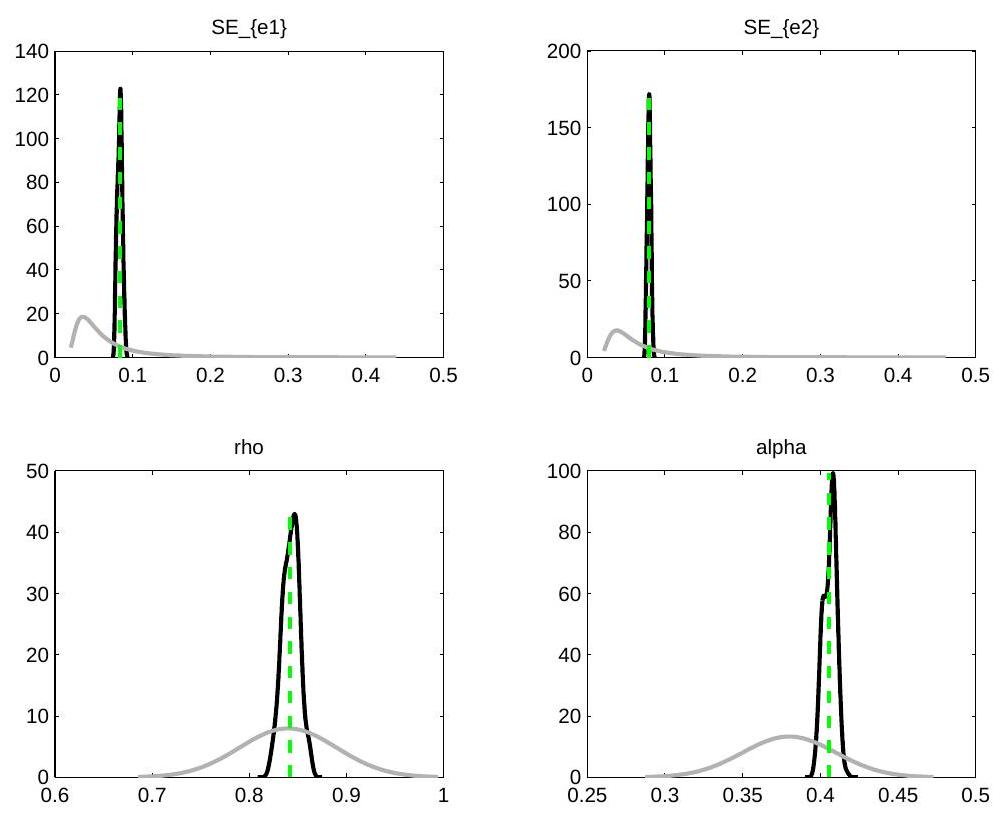
\includegraphics[width=\textwidth]{s03_03_posterior_legacy.jpg}
\captionsetup{labelformat=empty}
\caption{Figure 5: Prior v. Posterior Distribution}
\end{center}
\label{fig:s03-03-posterior-legacy}
\end{figure}


Given that there are two exogenous shock variables, we use two observables $\ln C_{1}$ and $\ln K_{2}$. The result of the estimation is summarized in Figure 5, where the posterior distribution (in the darker line) of each parameter is contrasted against the given prior distribution. The result can be compared to the true parameter values in Table 5.


\section{Fiscal policies in the growth model}
This section describes a suite of Dynare programs that implement the transition experiments performed in chapter 11 of Ljungqvist and Sargent (2004).

\subsection*{4.1 The model}
A deterministic growth model has inelastic labor supply, an exogenous stream of government expenditures, and several kinds of distorting taxes. All variables are as described in chapter 11 of Ljungqvist and Sargent (2004). A representative agent maximizes

$$
\sum_{t=0}^{\infty} \beta^{t} \frac{c_{t}^{1-\gamma}}{1-\gamma}, \quad \beta \in(0,1)
$$

Feasible allocations satisfy

$$
g_{t}+c_{t}+k_{t+1} \leq A k_{t}^{\alpha}+(1-\delta) k_{t} .
$$

Let $T_t$ denote a residual lump-sum tax (negative for a transfer), which finances spending net of distorting tax receipts. This closes the fiscal budget without altering the marginal conditions. The household budget constraint is

$$
\sum_{t=0}^{\infty}\left\{q_{t}\left(1+\tau_{c t}\right)c_t+\left(1-\tau_{i t}\right) q_{t}\left[k_{t+1}-(1-\delta) k_{t}\right]\right\} \leq \sum_{t=0}^{\infty}\left\{r_{t}\left(1-\tau_{k t}\right) k_{t}+w_{t}-q_t T_t\right\}
$$

and the government budget constraint is

$$
\sum_{t=0}^{\infty} q_{t} g_{t} \leq \sum_{t=0}^{\infty}\left\{\tau_{c t} q_{t} c_{t}-\tau_{i t} q_{t}\left[k_{t+1}-(1-\delta) k_{t}\right]+r_{t} \tau_{k t} k_{t}+q_t T_t\right\}
$$

The following conditions characterize an equilibrium:


\begin{align*}
c_{t} & =A k_{t}^{\alpha}+(1-\delta) k_{t}-k_{t+1}-g_{t}  \tag{7}\\
q_{t} & =\beta^{t} c_{t}^{-\gamma} /\left(1+\tau_{c t}\right)  \tag{8}\\
r_{t} / q_{t} & =A \alpha k_{t}^{\alpha-1}  \tag{9}\\
w_{t} / q_{t} & =A k_{t}^{\alpha}-k_{t} A \alpha k_{t}^{\alpha-1}  \tag{10}\\
R_{t+1} & =\frac{\left(1+\tau_{c t}\right)}{\left(1+\tau_{c t+1}\right)}\left[\frac{\left(1-\tau_{i t+1}\right)}{\left(1-\tau_{i t}\right)}(1-\delta)+\frac{\left(1-\tau_{k t+1}\right)}{\left(1-\tau_{i t}\right)} A \alpha k_{t+1}^{\alpha-1}\right]  \tag{11}\\
s_{t} / q_{t} & =\left(1-\tau_{k t}\right) A \alpha k_{t}^{\alpha-1}+(1-\delta)  \tag{12}\\
c_{t}^{-\gamma} & =\beta c_{t+1}^{-\gamma} R_{t+1} \tag{13}
\end{align*}


\paragraph{Dated prices and real plotting quantities.}
The ratios $r_t/q_t$, $w_t/q_t$ and $s_t/q_t$ express dated payoffs in current consumption-good units. They can be calculated directly from allocations; it is unnecessary to solve for a recursive $q_t$ and then divide by it. The dated-price recursion implied by (8) is
\[
q_t=\beta q_{t-1}
\left(\frac{c_t}{c_{t-1}}\right)^{-\gamma}
\frac{1+\tau_{c,t-1}}{1+\tau_{c,t}}.
\]
With constant consumption and taxes this becomes $q_t=\beta q_{t-1}$. For $0<\beta<1$ it has no positive constant steady-state level: imposing one gives $q=0$. This is not a unit root. Dropping $\beta$ removes the discount trend but gives $\widetilde q_t=\widetilde q_{t-1}$ at a constant allocation, leaving its level undetermined. The resulting unit root is not resolved merely by calling the variable a stationary kernel. This corrects the explanation in the preserved 2025 training file.

The section examples therefore solve allocations first. Their optional commented epilogues calculate real factor prices and the Euler-implied return without a $q$ state. The full-output files include those observables explicitly. Dated prices are reconstructed only when needed, using the normalization
\[
\frac{q_t}{q_0}=\beta^t
\left(\frac{c_t}{c_0}\right)^{-\gamma}
\frac{1+\tau_{c,0}}{1+\tau_{c,t}}.
\]
The one-period pricing factor is $q_{t+1}/q_t$; it retains $\beta$. A detrended price level is not itself this one-period factor. See \path{notes/q_and_auxiliaries.md} for the implementation mapping and the 2025 comment erratum.

Because the other endogenous variables can be expressed as functions of $k_{t}$ and $c_{t}$, in the programs below we use only a subset of the equilibrium conditions to compute equilibrium paths.

\subsection*{4.2 Parameter values}
We set the parameters and the baseline values of the exogenous variables at values set in chapter 11 of Ljungqvist and Sargent (2004), as described in the following table are taken from RMT2.

\begin{center}
\begin{tabular}{cc}
\hline
Parameter/exogenous variable & Values \\
\hline
$\beta$ & 0.95 \\
$\delta$ & 0.2 \\
$A$ & 1 \\
$\alpha$ & 0.33 \\
$\gamma$ & 2 \\
$g$ & 0.2 \\
$\tau_{c}$ & 0 \\
$\tau_{i}$ & 0 \\
$\tau_{k}$ & 0 \\
\hline
\end{tabular}
\end{center}

\subsection*{4.3 Transition experiments}
\subsection*{4.3.1 A permanent increase in g (Figure 11.3.1).}
The Dynare code below implements the experiment associated with Figure 11.3.1. which looks at the impact of a permanent increase of 0.2 in $g$ at $\mathrm{t}=10$.\\

\lstinputlisting{Code/sections/s04_03_01_g.mod}

\begin{figure}[!htbp]
\begin{center}
  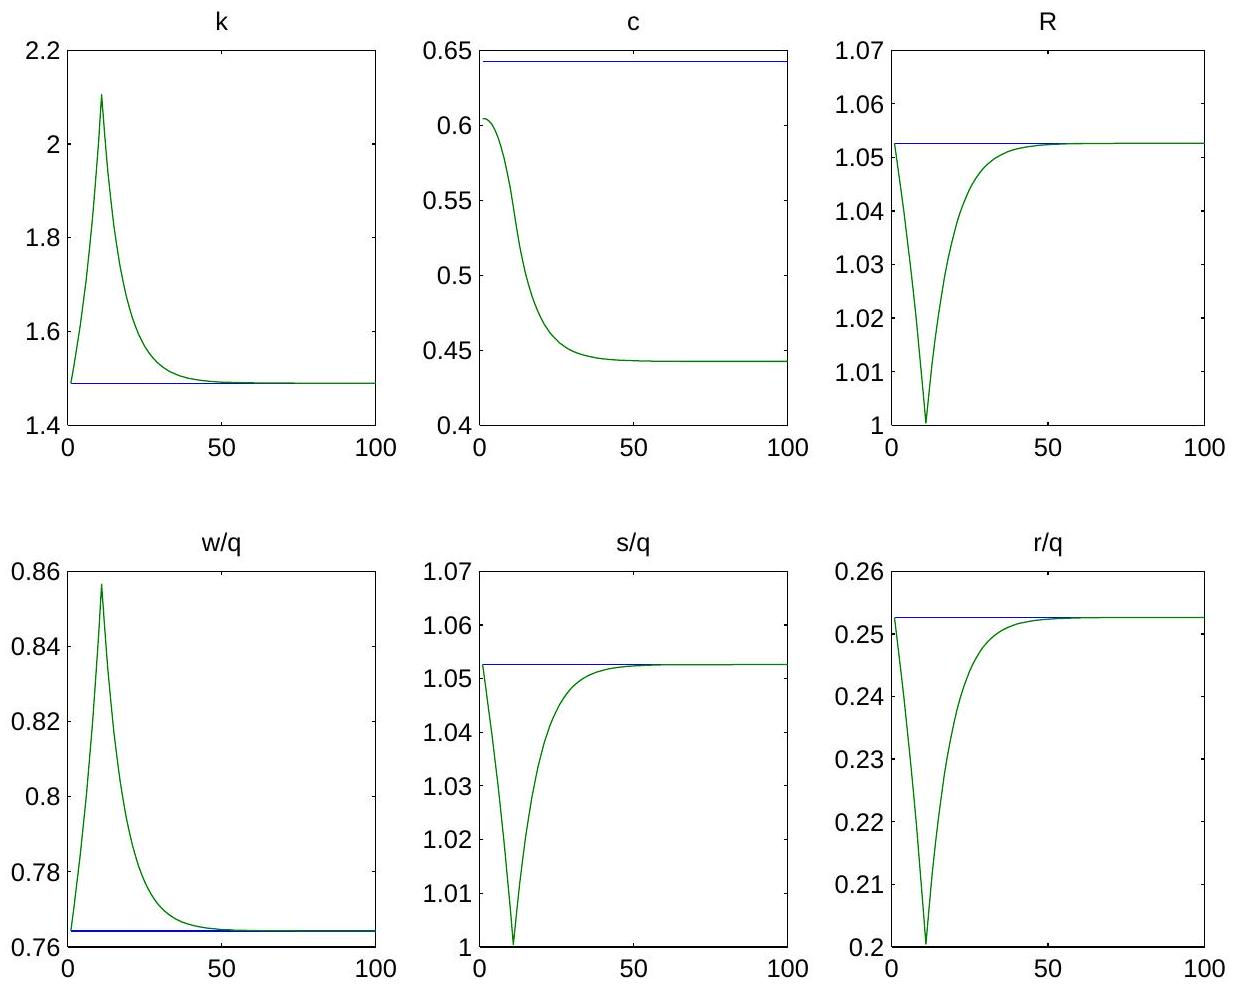
\includegraphics[width=\textwidth]{s04_03_01_g_legacy.jpg}
\captionsetup{labelformat=empty}
\caption{Figure 6: A permanent increase of g (Figure 11.3.1).}
\end{center}
\label{fig:s04-03-01-g-legacy}
\end{figure}


The following figure shows the path of the endogenous variables along the transition to the new steady state.\\
The remaining experiments each have a complete, independently runnable file.

\subsection*{4.3.2 A permanent increase in $\tau_{c}$ (Figure 11.3.2).}
A permanent increase of $\tau_{c}$ at $\mathrm{t}=10$ of 20 percentage points. (Figure 11.3.2)

\lstinputlisting{Code/sections/s04_03_02_tauc.mod}

\begin{figure}[!htbp]
\begin{center}
  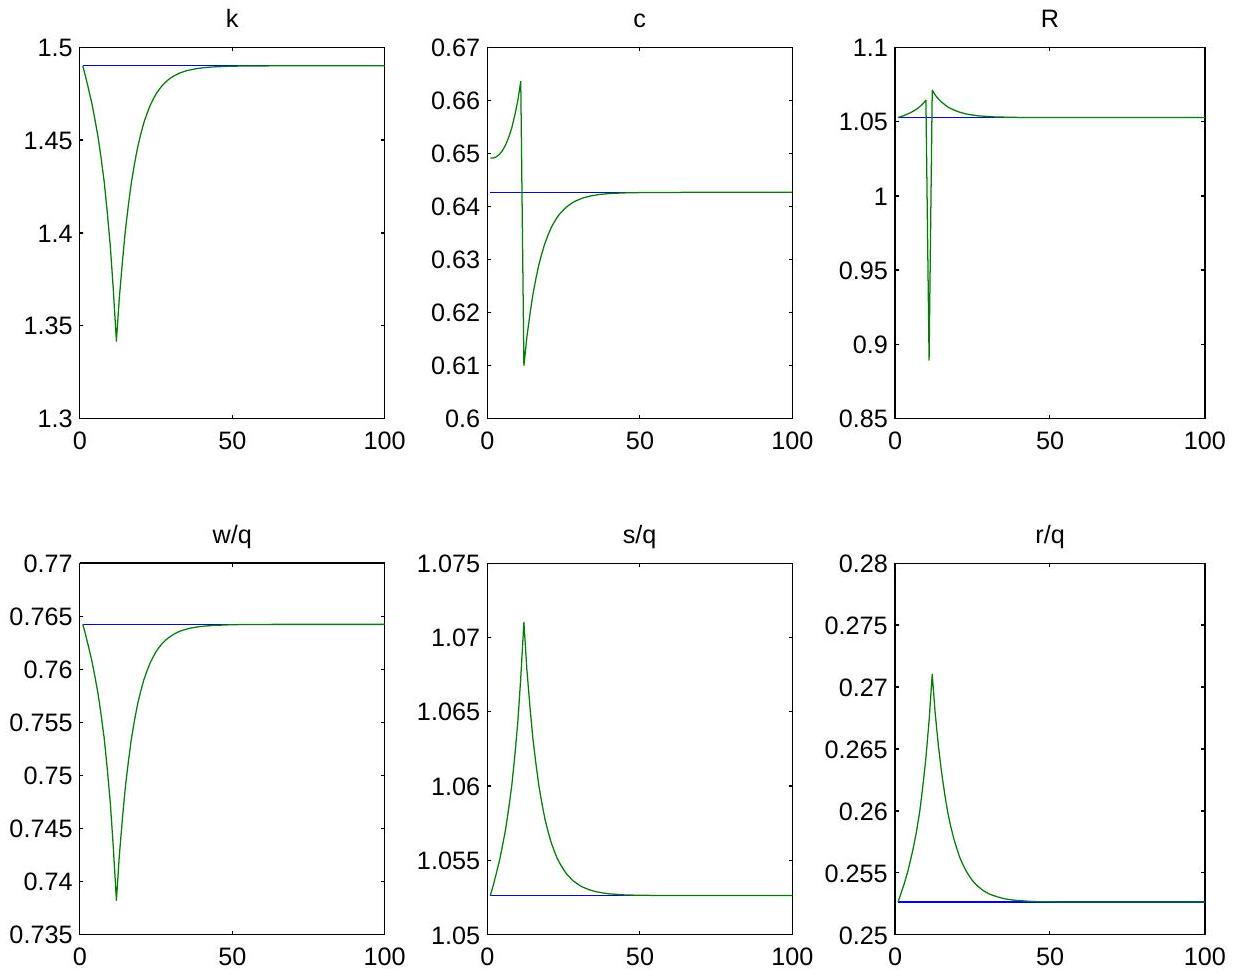
\includegraphics[width=\textwidth]{s04_03_02_tauc_legacy.jpg}
\captionsetup{labelformat=empty}
\caption{Figure 7: A permanent increase of $\tau_c$ (Figure 11.3.2).}
\end{center}
\label{fig:s04-03-02-tauc-legacy}
\end{figure}


\subsection*{4.3.3 A permanent increase in $\tau_{i}$ (Figure 11.5.1).}
A permanent increase of $\tau_{i}$ at $\mathrm{t}=10$ of 20 percentage points. (Figure 11.5.1)

\lstinputlisting{Code/sections/s04_03_03_taui.mod}

\begin{figure}[!htbp]
\begin{center}
  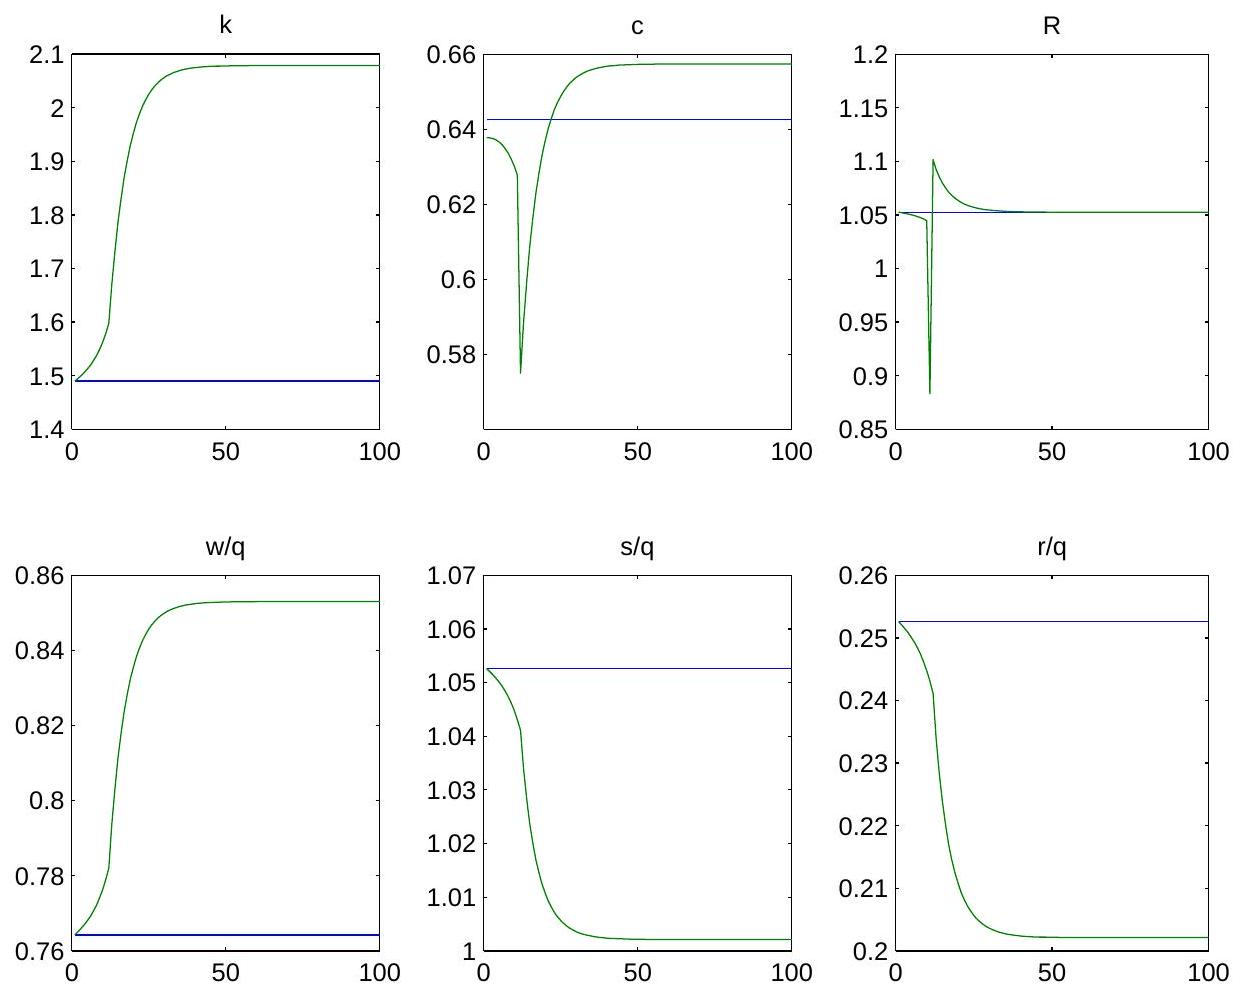
\includegraphics[width=\textwidth]{s04_03_03_taui_legacy.jpg}
\captionsetup{labelformat=empty}
\caption{Figure 8: A permanent increase of $\tau_i$ (Figure 11.5.1).}
\end{center}
\label{fig:s04-03-03-taui-legacy}
\end{figure}


\subsection*{4.3.4 A permanent increase in $\tau_{k}$ (Figure 11.5.2).}
A permanent increase of $\tau_{k}$ at $\mathrm{t}=10$ of 20 percentage points. (Figure 11.5.2)

\lstinputlisting{Code/sections/s04_03_04_tauk.mod}

\begin{figure}[!htbp]
\begin{center}
  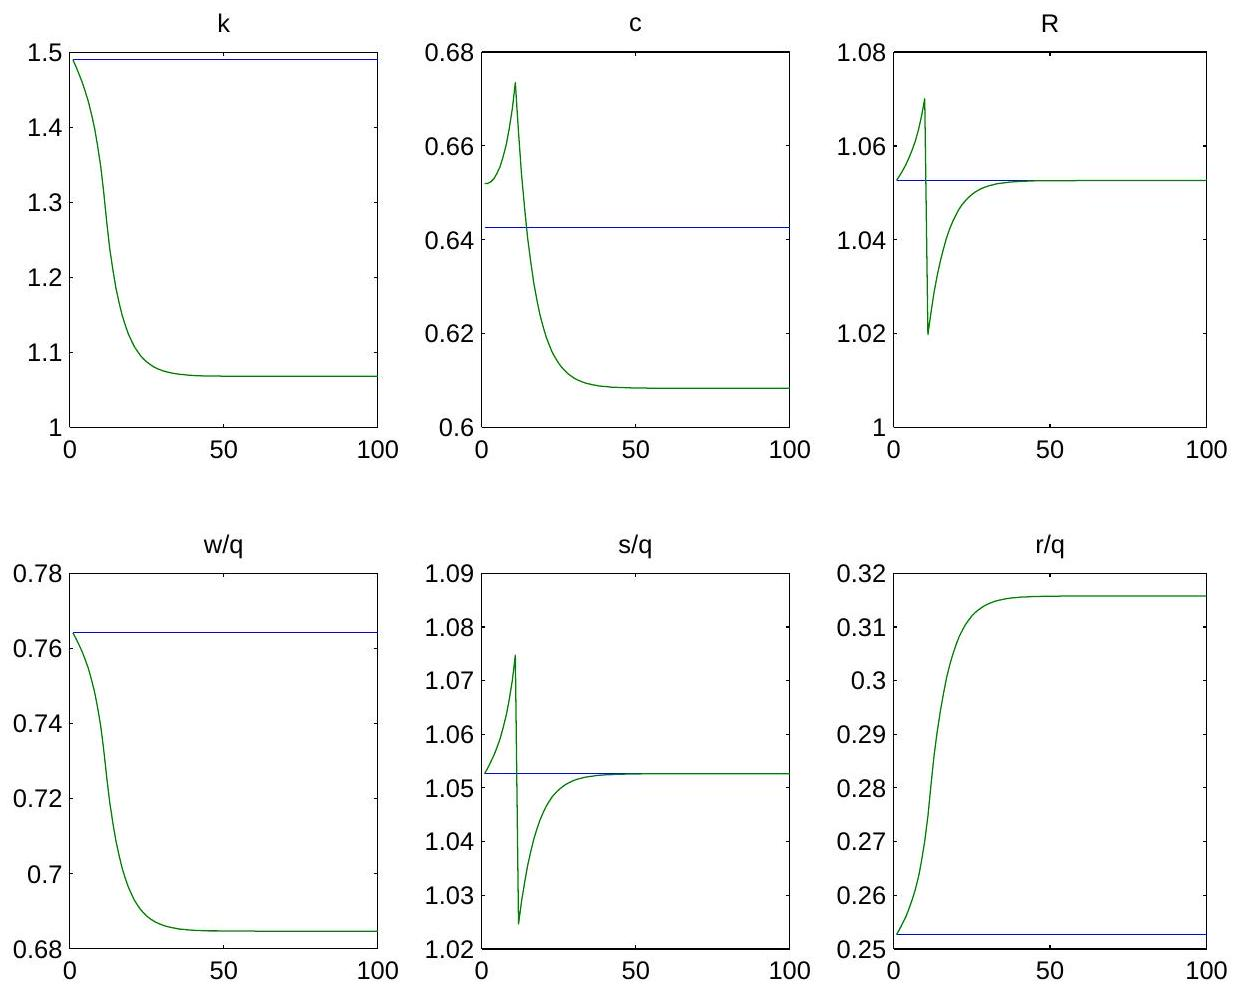
\includegraphics[width=\textwidth]{s04_03_04_tauk_legacy.jpg}
\captionsetup{labelformat=empty}
\caption{Figure 9: A permanent increase of $\tau_k$ (Figure 11.5.2).}
\end{center}
\label{fig:s04-03-04-tauk-legacy}
\end{figure}


\subsection*{4.3.5 One time increase in g (Figure 11.7.1).}
A one time pulse of $g$ at $\mathrm{t}=10$ of 0.2 . (Figure 11.7.1)

\lstinputlisting{Code/sections/s04_03_05_g.mod}

\begin{figure}[!htbp]
\begin{center}
  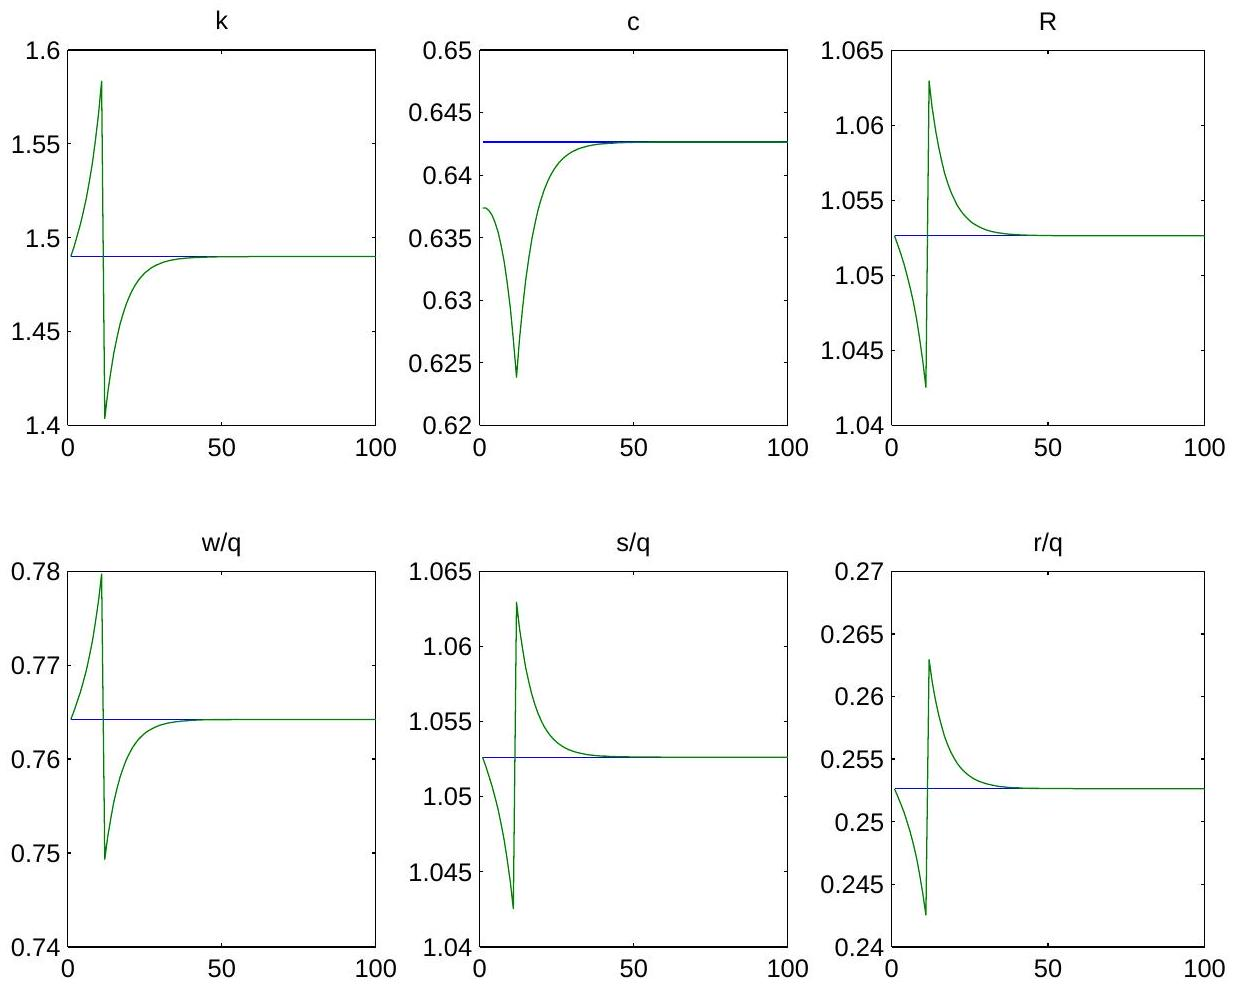
\includegraphics[width=\textwidth]{s04_03_05_g_legacy.jpg}
\captionsetup{labelformat=empty}
\caption{Figure 10: One time increase of g (Figure 11.7.1).}
\end{center}
\label{fig:s04-03-05-g-legacy}
\end{figure}


\subsection*{4.3.6 One time increase in $\tau_{i}$ (Figure 11.7.2).}
A one time pulse of $\tau_{i}$ at $\mathrm{t}=10$ of 20 percentage points. (Figure 11.7.2)

\lstinputlisting{Code/sections/s04_03_06_taui.mod}

\begin{figure}[!htbp]
\begin{center}
  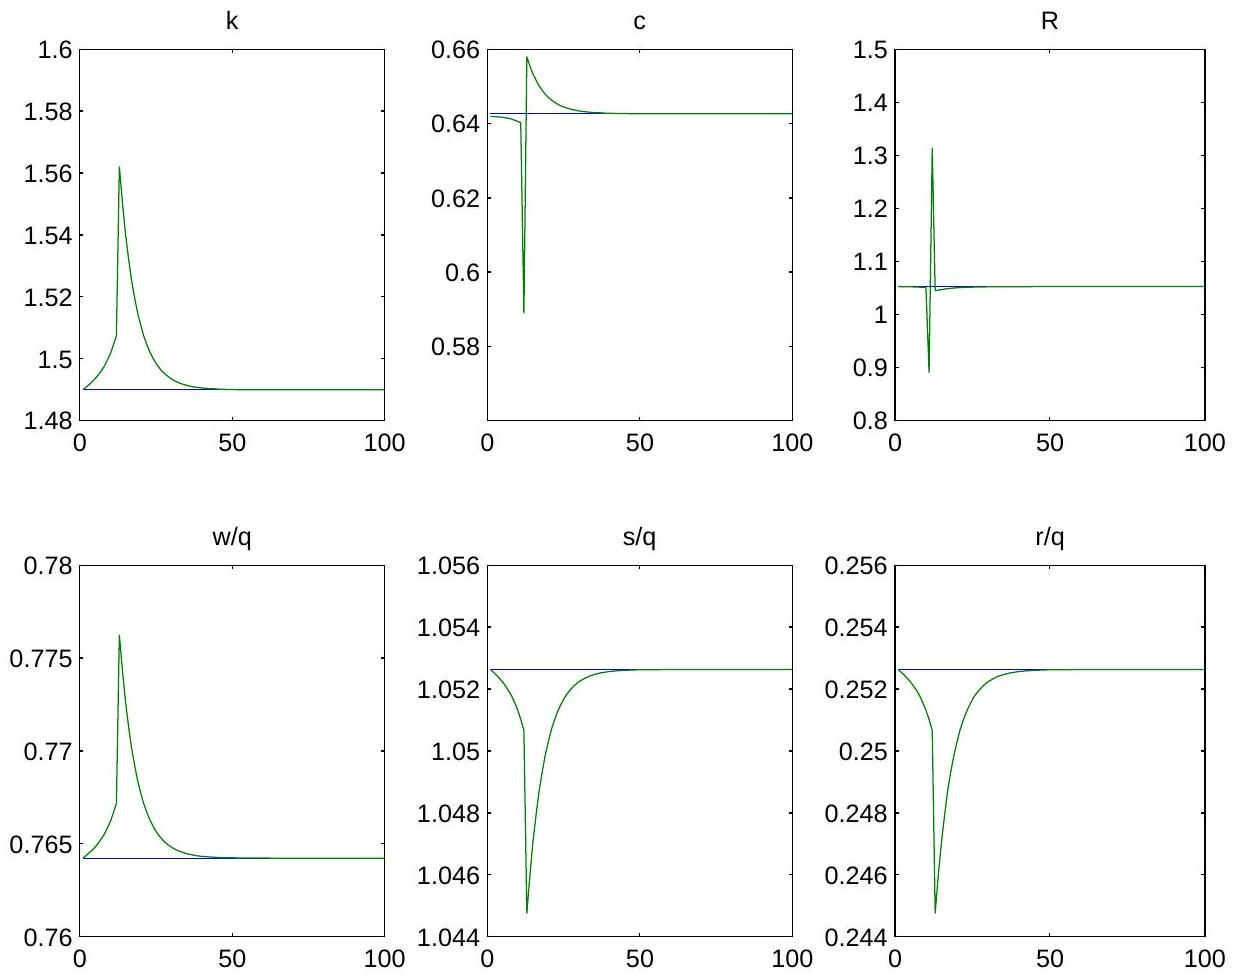
\includegraphics[width=\textwidth]{s04_03_06_taui_legacy.jpg}
\captionsetup{labelformat=empty}
\caption{Figure 11: One time increase of $\tau_i$ (Figure 11.7.2).}
\end{center}
\label{fig:s04-03-06-taui-legacy}
\end{figure}


\section{Fiscal policies in the growth model, 2.0}
This section describes a suite of Dynare programs that implement the transition experiments performed in chapter 11 of Ljungqvist and Sargent (2012).

\subsection*{5.1 The model with inelastic labor supply}
A deterministic growth model has inelastic labor supply, an exogenous stream of government expenditures, and several kinds of distorting taxes. All variables are as described in chapter 11 of Ljungqvist and Sargent (2012). A representative agent maximizes

$$
\sum_{t=0}^{\infty} \beta^{t} \frac{c_{t}^{1-\gamma}}{1-\gamma}, \quad \beta \in(0,1)
$$

Feasible allocations satisfy

$$
g_{t}+c_{t}+k_{t+1} \leq A k_{t}^{\alpha}+(1-\delta) k_{t}
$$

Let $T_t$ denote a residual lump-sum tax (negative for a transfer), which finances spending net of distorting tax receipts. This closes the fiscal budget without altering the marginal conditions. The household budget constraint is

$$
\sum_{t=0}^{\infty}\left\{q_{t} c_{t}\left(1+\tau_{c t}\right)+q_{t}\left[k_{t+1}-(1-\delta) k_{t}\right]\right\} \leq \sum_{t=0}^{\infty} q_{t}\left\{\eta_{t}\left(1-\tau_{k t}\right) k_{t}+w_{t}-T_t\right\}
$$

and the government budget constraint is

$$
\sum_{t=0}^{\infty} q_{t} g_{t} \leq \sum_{t=0}^{\infty} q_{t}\left\{\tau_{c t} c_{t}+\tau_{k t} \eta_{t} k_{t}+T_t\right\}
$$

The following conditions characterize an equilibrium:


\begin{align*}
c_{t} & =A k_{t}^{\alpha}+(1-\delta) k_{t}-k_{t+1}-g_{t}  \tag{14}\\
q_{t} & =\beta^{t} c_{t}^{-\gamma} /\left(1+\tau_{c t}\right)  \tag{15}\\
\eta_{t} & =A \alpha k_{t}^{\alpha-1}  \tag{16}\\
w_{t} & =A k_{t}^{\alpha}-k_{t} A \alpha k_{t}^{\alpha-1}  \tag{17}\\
\bar{R}_{t+1} & =\frac{\left(1+\tau_{c t}\right)}{\left(1+\tau_{c t+1}\right)}\left[(1-\delta)+\left(1-\tau_{k t+1}\right) A \alpha k_{t+1}^{\alpha-1}\right]  \tag{18}\\
c_{t}^{-\gamma} & =\beta c_{t+1}^{-\gamma} \bar{R}_{t+1} \tag{19}
\end{align*}


Because the other endogenous variables can be expressed as functions of $k_{t}$ and $c_{t}$, in the programs below we use only a subset of the equilibrium conditions to compute equilibrium paths.

\subsection*{5.2 Parameter values}
We set the parameters and the baseline values of the exogenous variables at values set in chapter 11 of Ljungqvist and Sargent (2012), as described in the following table are taken from RMT3.

\begin{center}
\begin{tabular}{cc}
\hline
Parameter/exogenous variable & Values \\
\hline
$\beta$ & 0.95 \\
$\delta$ & 0.2 \\
$A$ & 1 \\
$\alpha$ & 0.33 \\
$\gamma$ & 2 \\
$g$ & 0.2 \\
$\tau_{c}$ & 0 \\
$\tau_{k}$ & 0 \\
\hline
\end{tabular}
\end{center}

\subsection*{5.3 Transition experiments}
\subsection*{5.3.1 Foreseen once-and-for-all increase in g (Figure 11.6.1).}
The Dynare code below implements the experiment associated with Figure 11.6.1. which looks at the impact of a foreseen once-for-and-all increase of 0.2 in g at $t=10$.

\lstinputlisting{Code/sections/s05_03_01_g.mod}

\begin{figure}[!htbp]
\begin{center}
  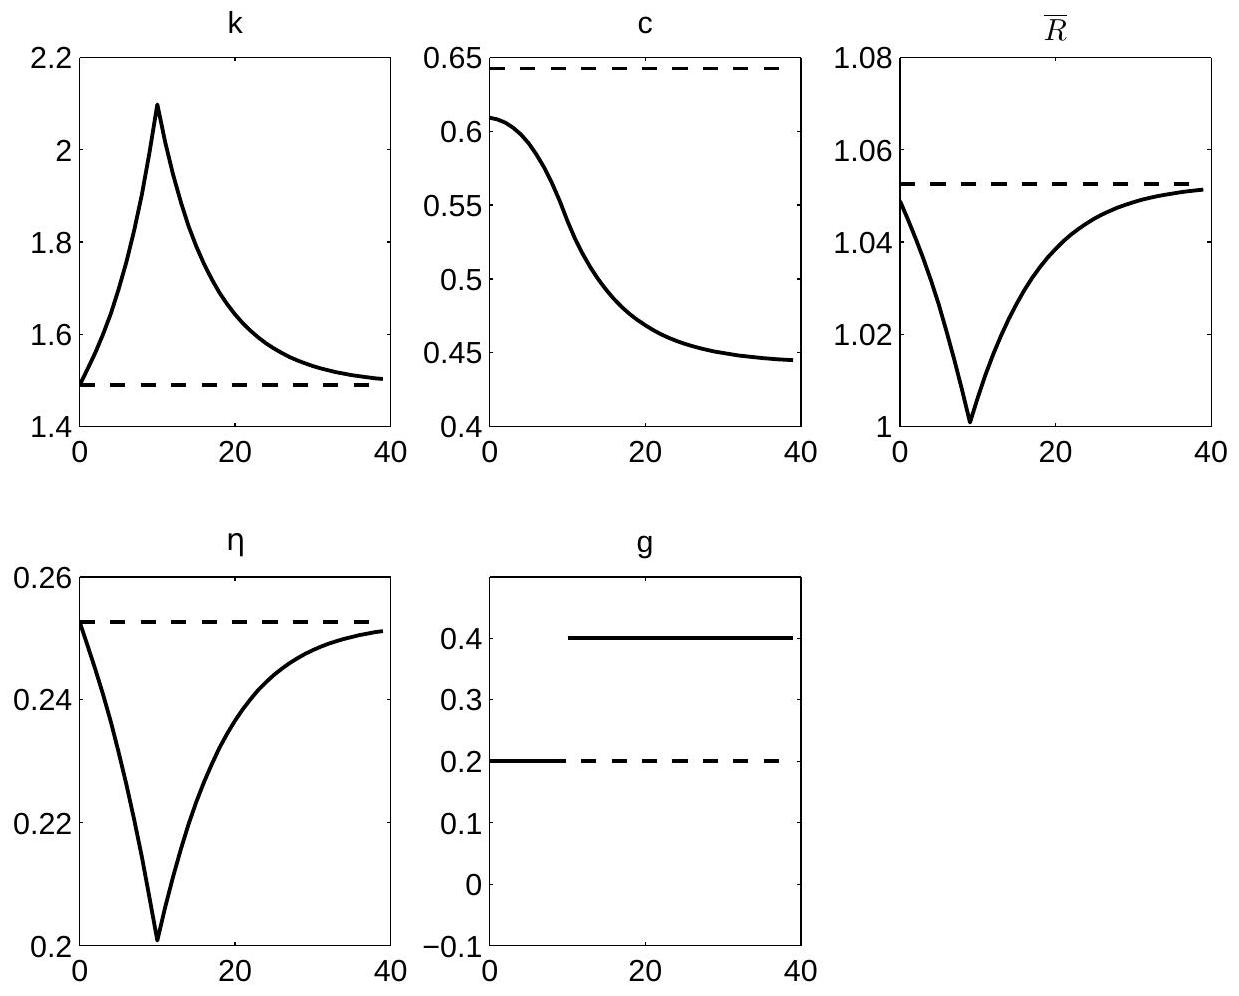
\includegraphics[width=\textwidth]{s05_03_01_g_legacy.jpg}
\captionsetup{labelformat=empty}
\caption{Figure 12: Foreseen once-and-for-all increase in g at $t=10$ (Figure 11.6.1).}
\end{center}
\label{fig:s05-03-01-g-legacy}
\end{figure}


The following figure shows the path of the endogenous variables along the transition to the new steady state.\\
The remaining experiments each have a complete, independently runnable file.

\subsection*{5.3.2 Foreseen once-and-for-all increase in $\tau_{c}$ (Figure 11.6.4).}
A foreseen once-and-for-all increase in $\tau_{c}$ at $t=10$ of 20 percentage points.(Figure 11.6.4)

\lstinputlisting{Code/sections/s05_03_02_tauc.mod}

\begin{figure}[!htbp]
\begin{center}
  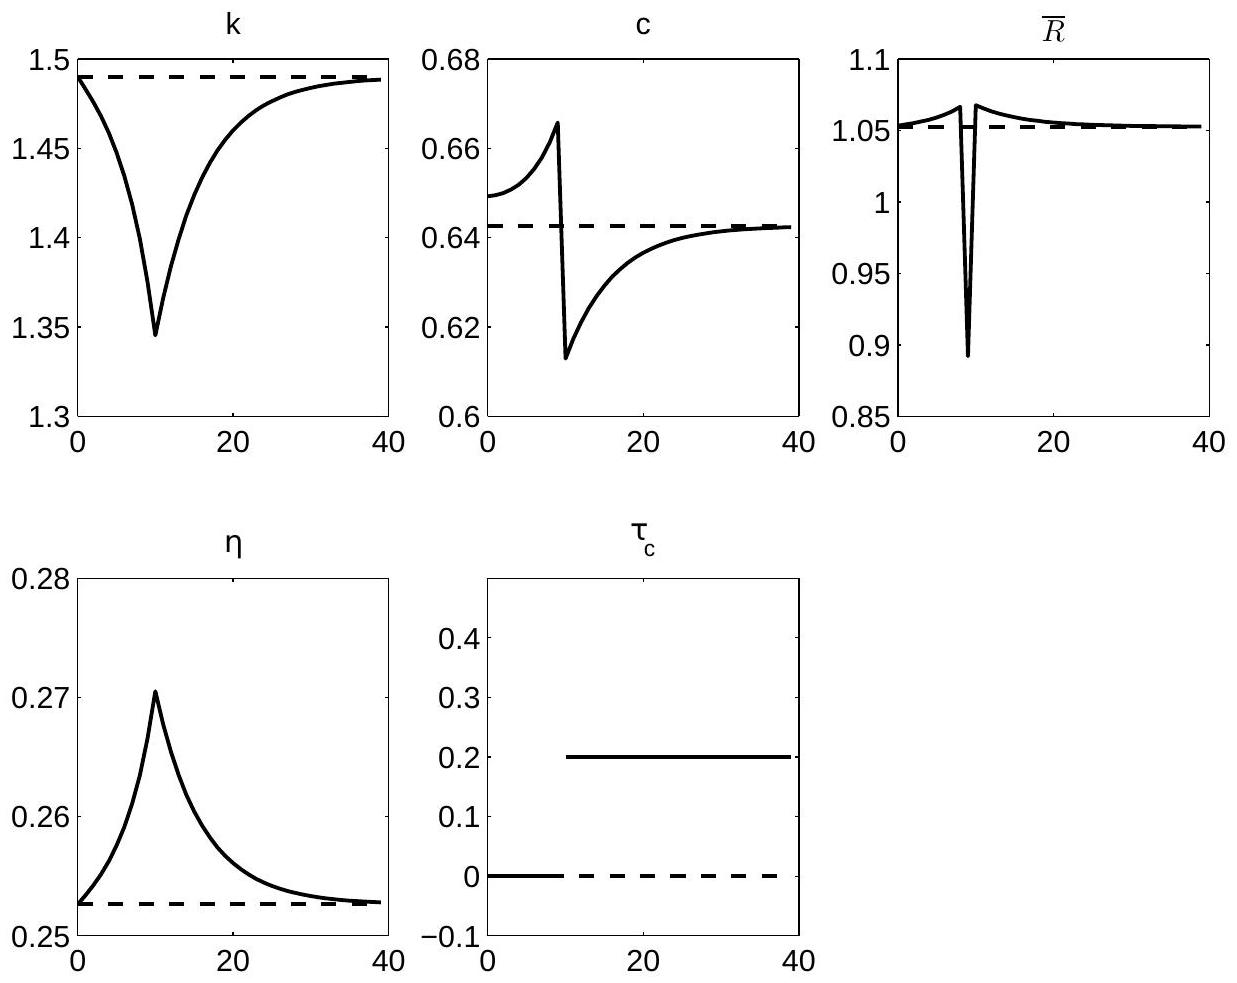
\includegraphics[width=\textwidth]{s05_03_02_tauc_legacy.jpg}
\captionsetup{labelformat=empty}
\caption{Figure 13: Foreseen once-and-for-all increase in $\tau_c$ at $t=10$ (Figure 11.6.4).}
\end{center}
\label{fig:s05-03-02-tauc-legacy}
\end{figure}


\subsection*{5.3.3 Foreseen once-and-for-all increase in $\tau_{k}$ (Figure 11.6.5).}
A foreseen once-and-for-all increase in $\tau_{k}$ at $t=10$ of 20 percentage points. (Figure 11.6.5)

\lstinputlisting{Code/sections/s05_03_03_tauk.mod}

\begin{figure}[!htbp]
\begin{center}
  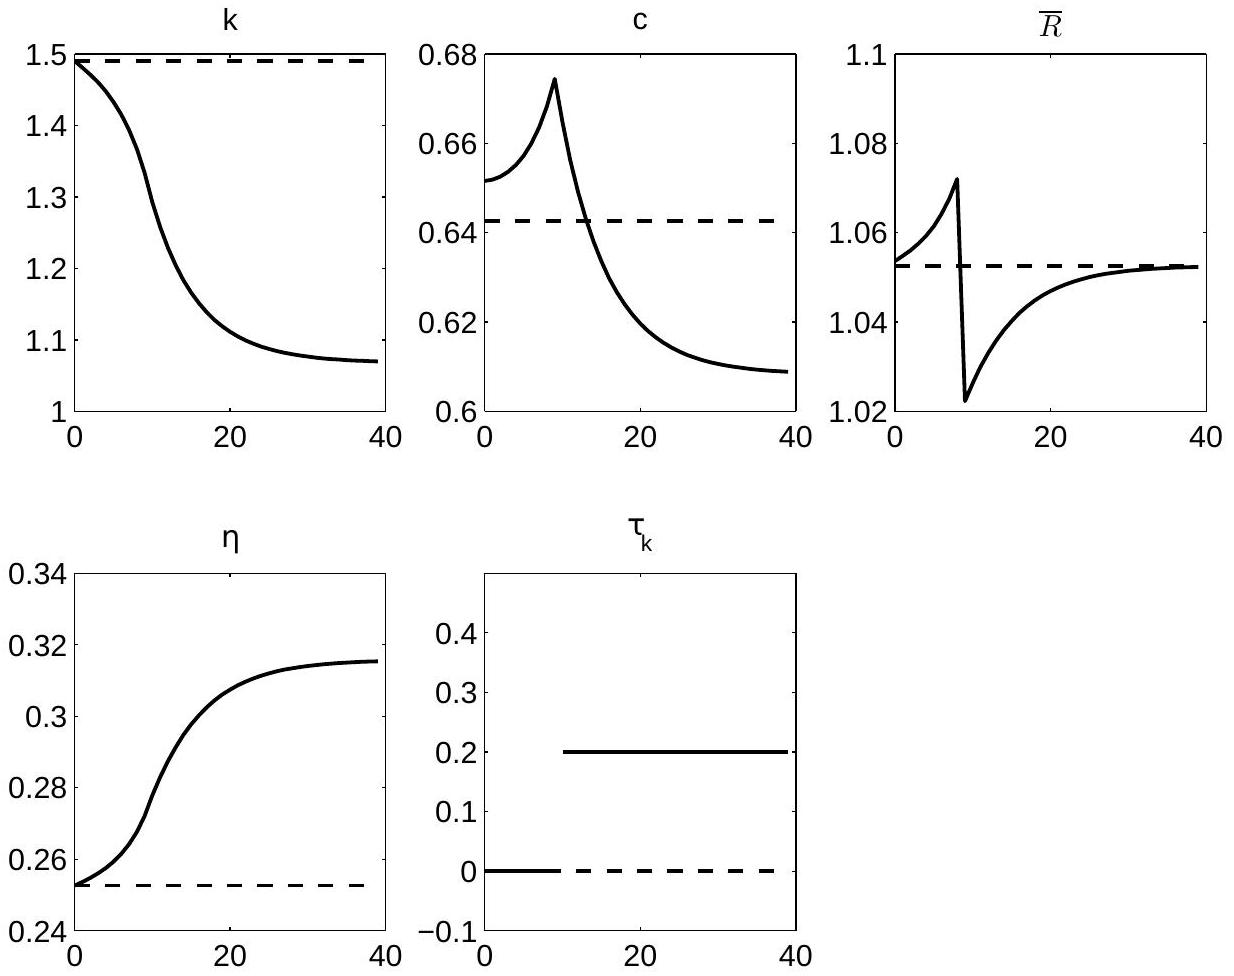
\includegraphics[width=\textwidth]{s05_03_03_tauk_legacy.jpg}
\captionsetup{labelformat=empty}
\caption{Figure 14: Foreseen once-and-for-all foreseen increase in $\tau_k$ at $t=10$ (Figure 11.6.5).}
\end{center}
\label{fig:s05-03-03-tauk-legacy}
\end{figure}


\subsection*{5.3.4 Foreseen one-time pulse increase in g (Figure 11.6.6).}
A foreseen one-time pulse of $g$ at $t=10$ of 0.2 . (Figure 11.6.6)

\lstinputlisting{Code/sections/s05_03_04_g.mod}

\begin{figure}[!htbp]
\begin{center}
  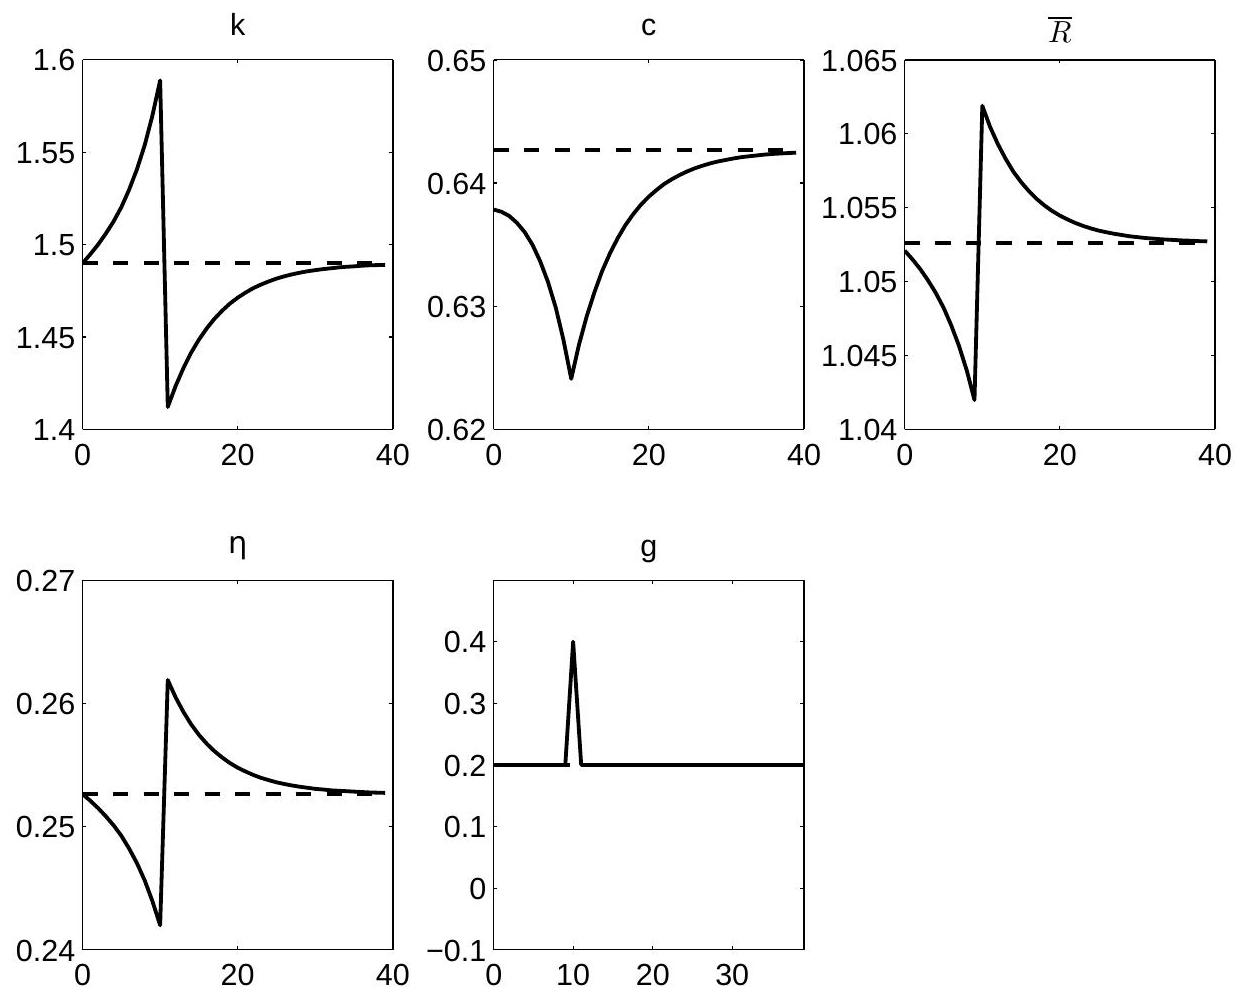
\includegraphics[width=\textwidth]{s05_03_04_g_legacy.jpg}
\captionsetup{labelformat=empty}
\caption{Figure 15: Foreseen one-time pulse increase in g at $t=10$ (Figure 11.6.6).}
\end{center}
\label{fig:s05-03-04-g-legacy}
\end{figure}


\subsection*{5.3.5 Foreseen once-and-for-all increase $\mathbf{g}$ at $\mathbf{t}=10$ for two economies (Figure 11.6.2).}
Responses to a foreseen increase in $g$ at $t=10$ for two economies, the original economy with $\gamma=2$ and an otherwise identical economy with $\gamma=.2$ (Figure 11.6.2).

Compare the following low-curvature economy with \texttt{s05\_03\_01\_g.mod} ($\gamma=2$).
\lstinputlisting{Code/sections/s05_03_05_g_gamma02.mod}

\begin{figure}[!htbp]
\begin{center}
  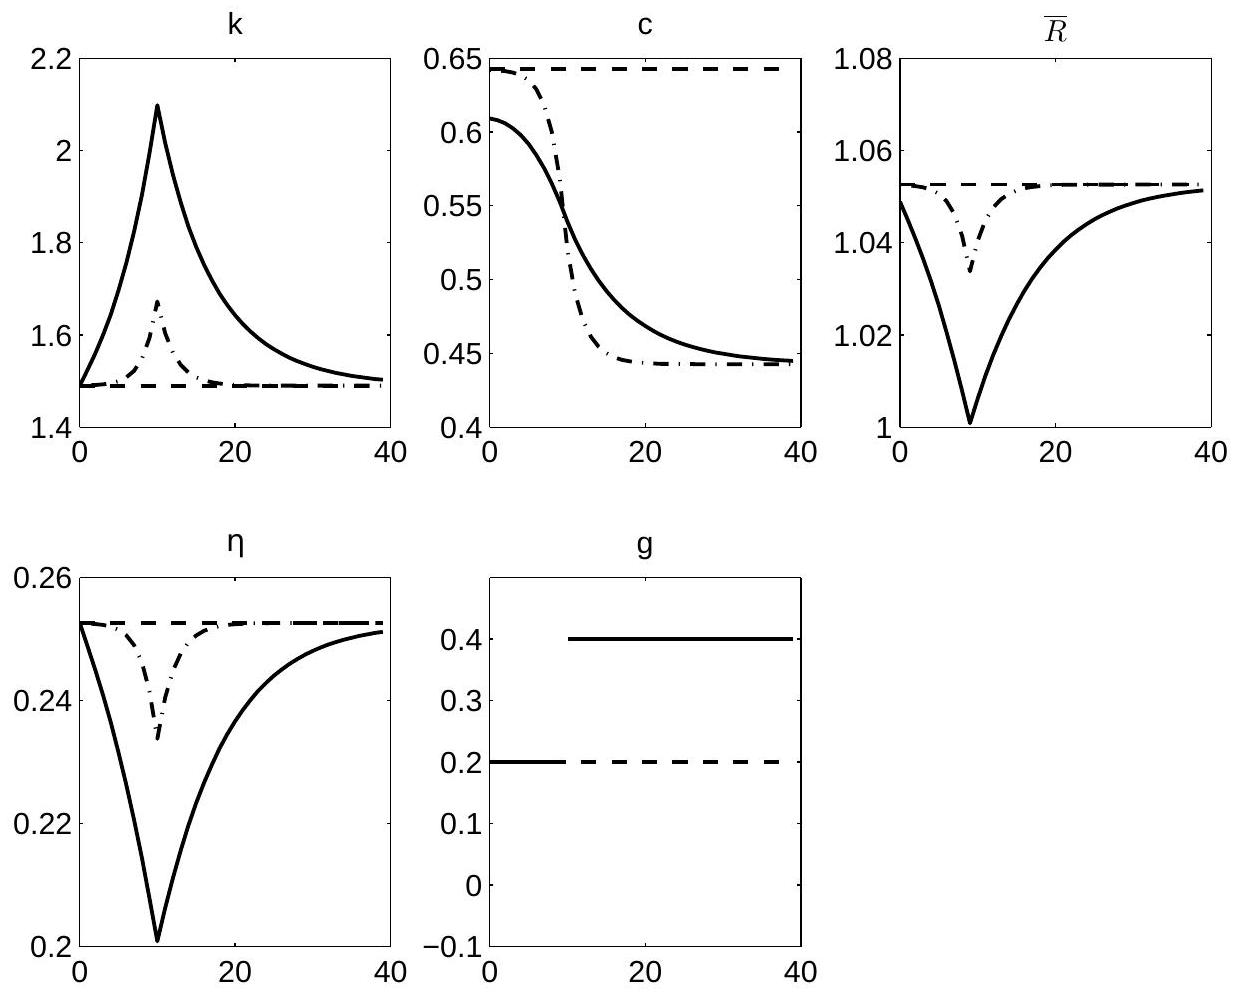
\includegraphics[width=\textwidth]{s05_03_05_g_gamma_comparison_legacy.jpg}
\captionsetup{labelformat=empty}
\caption{Figure 16: Response to foreseen once-and-for-all increase in g at $t=10$. The solid line is for $\gamma=2$, while the dashed-dotted line is for $\gamma=.2$ (Figure 11.6.2).}
\end{center}
\label{fig:s05-03-05-g-gamma-comparison-legacy}
\end{figure}


\subsection*{5.3.6 Impact of an foreseen once-and-for-all increase in g on yield curves (Figure 11.6.3).}
Impact of an foreseen once-and-for-all increase in $g$ at $t=10$ on yield curves. For this section we use normalized dated prices (including the consumption-tax wedge, which is constant in this spending experiment) and continuously compounded yields


\begin{align*}
q_{t}/q_0 & =\beta^{t}\left(\frac{c_t}{c_0}\right)^{-\gamma}\frac{1+\tau_{c,0}}{1+\tau_{c,t}}  \tag{20}\\
y_{i, t} & =-\frac{1}{i} \log \left(\frac{q_{t+i}}{q_{t}}\right) \tag{21}
\end{align*}


\lstinputlisting{Code/sections/s05_03_06_yields.mod}

\begin{figure}[!htbp]
\begin{center}
  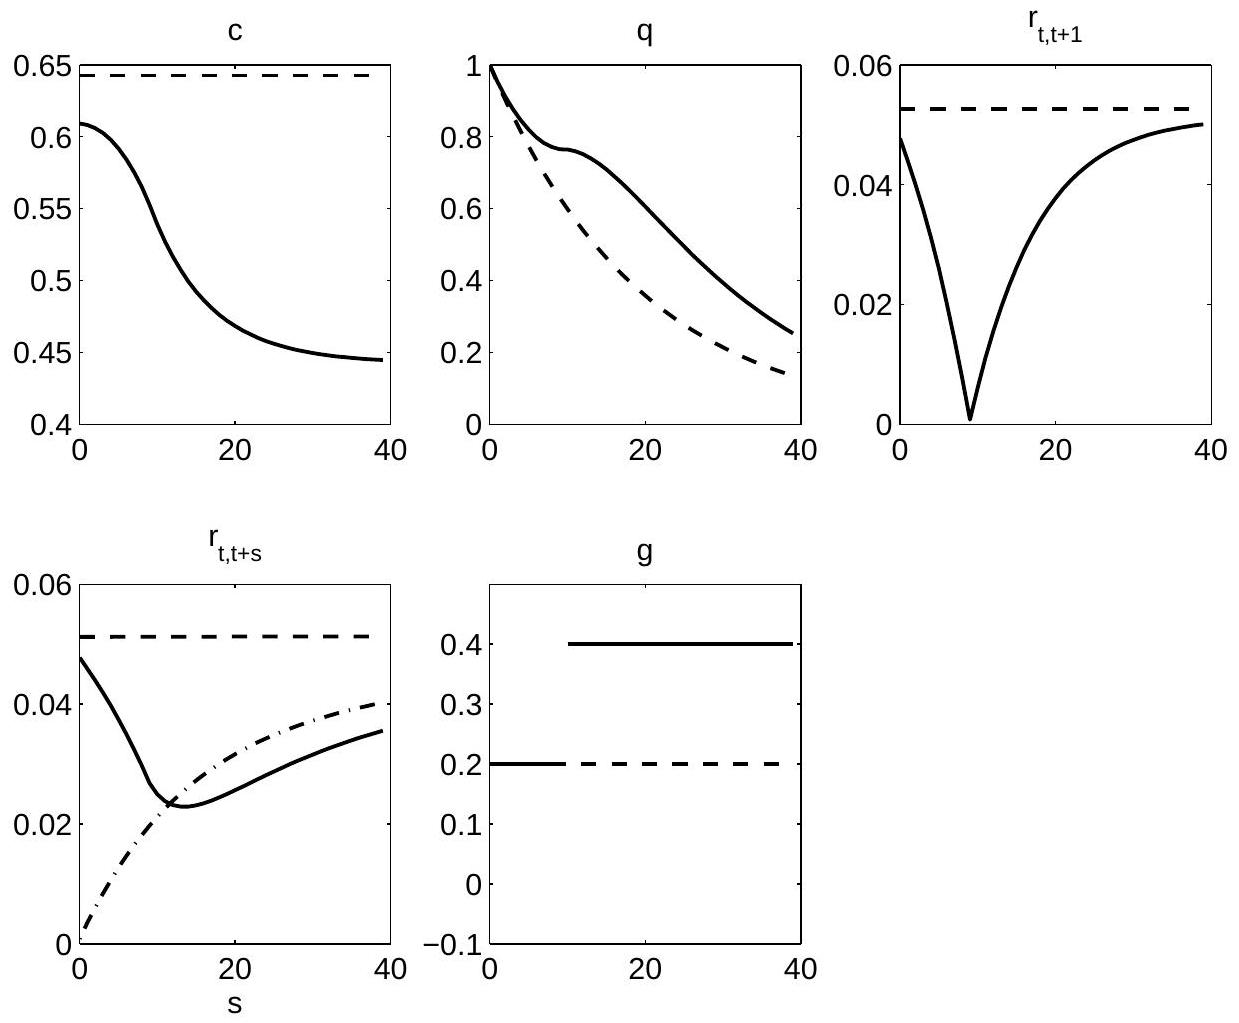
\includegraphics[width=\textwidth]{s05_03_06_yields_legacy.jpg}
\captionsetup{labelformat=empty}
\caption{Figure 17: Response to foreseen once-and-for-all increase in g at $t=10$. Yield curves for $t=0$ (solid line), $t=10$ (dashdotted line) and $t=60$ (dashed line); term to maturity is on the x axis for the yield curve, time for the other panels (Figure 11.6.3).}
\end{center}
\label{fig:s05-03-06-yields-legacy}
\end{figure}


\subsection*{5.4 The model with elastic labor supply}
In this section we modify the previous model by allowing for elastic labor supply. Now the representative agent maximizes

$$
\sum_{t=0}^{\infty} \beta^{t} [\log c_t+B(1-n_t)], \quad \beta \in(0,1)
$$

where B is substantially greater than 1 to assure an interior solution $n \in(0,1)$ for labor supply. Feasible allocations satisfy

$$
g_{t}+c_{t}+k_{t+1} \leq A k_{t}^{\alpha} n_{t}^{1-\alpha}+(1-\delta) k_{t} .
$$

Let $T_t$ denote a residual lump-sum tax (negative for a transfer), which finances spending net of distorting tax receipts. This closes the fiscal budget without altering the marginal conditions. The household budget constraint is

$$
\sum_{t=0}^{\infty}\left\{q_{t}\left(1+\tau_{c t}\right)c_t+q_{t}\left[k_{t+1}-(1-\delta) k_{t}\right]\right\} \leq \sum_{t=0}^{\infty} q_{t}\left\{\eta_{t}\left(1-\tau_{k t}\right) k_{t}+w_{t}n_t\left(1-\tau_{n t}\right)-T_t\right\}
$$

and the government budget constraint is

$$
\sum_{t=0}^{\infty} q_{t} g_{t} \leq \sum_{t=0}^{\infty} q_{t}\left\{\tau_{c t} c_{t}+\tau_{k t} \eta_{t} k_{t}+\tau_{n t} n_{t} w_{t}+T_t\right\}
$$

The following conditions characterize the endogenous variables in the model equilibrium:


\begin{align*}
c_{t} & =A k_{t}^{\alpha} n_{t}^{1-\alpha}+(1-\delta) k_{t}-k_{t+1}-g_{t}  \tag{22}\\
c_{t}^{-1} & =\beta c_{t+1}^{-1}\left(\frac{1+\tau_{c t}}{1+\tau_{c t+1}}\right)\left[(1-\delta)+\left(1-\tau_{k t+1}\right) A \alpha k_{t+1}^{\alpha-1} n_{t+1}^{1-\alpha}\right]  \tag{23}\\
B c_{t}\left(1+\tau_{c t}\right) & =\left(1-\tau_{n t}\right)\left[(1-\alpha) A k_{t}^{\alpha} n_{t}^{-\alpha}\right] \tag{24}
\end{align*}


\subsection*{5.4.1 Elastic Labor supply : Unforseen once-and-for-all increase in $\mathbf{g}$ at $\mathbf{t}=\mathbf{0}$ (Figure 11.9.1).}
An unforeseen once-and-for-all increase in g from 0.2 to 0.4 at $t=0$ (Figure 11.9.1).

\lstinputlisting{Code/sections/s05_04_01_g.mod}

\begin{figure}[!htbp]
\begin{center}
  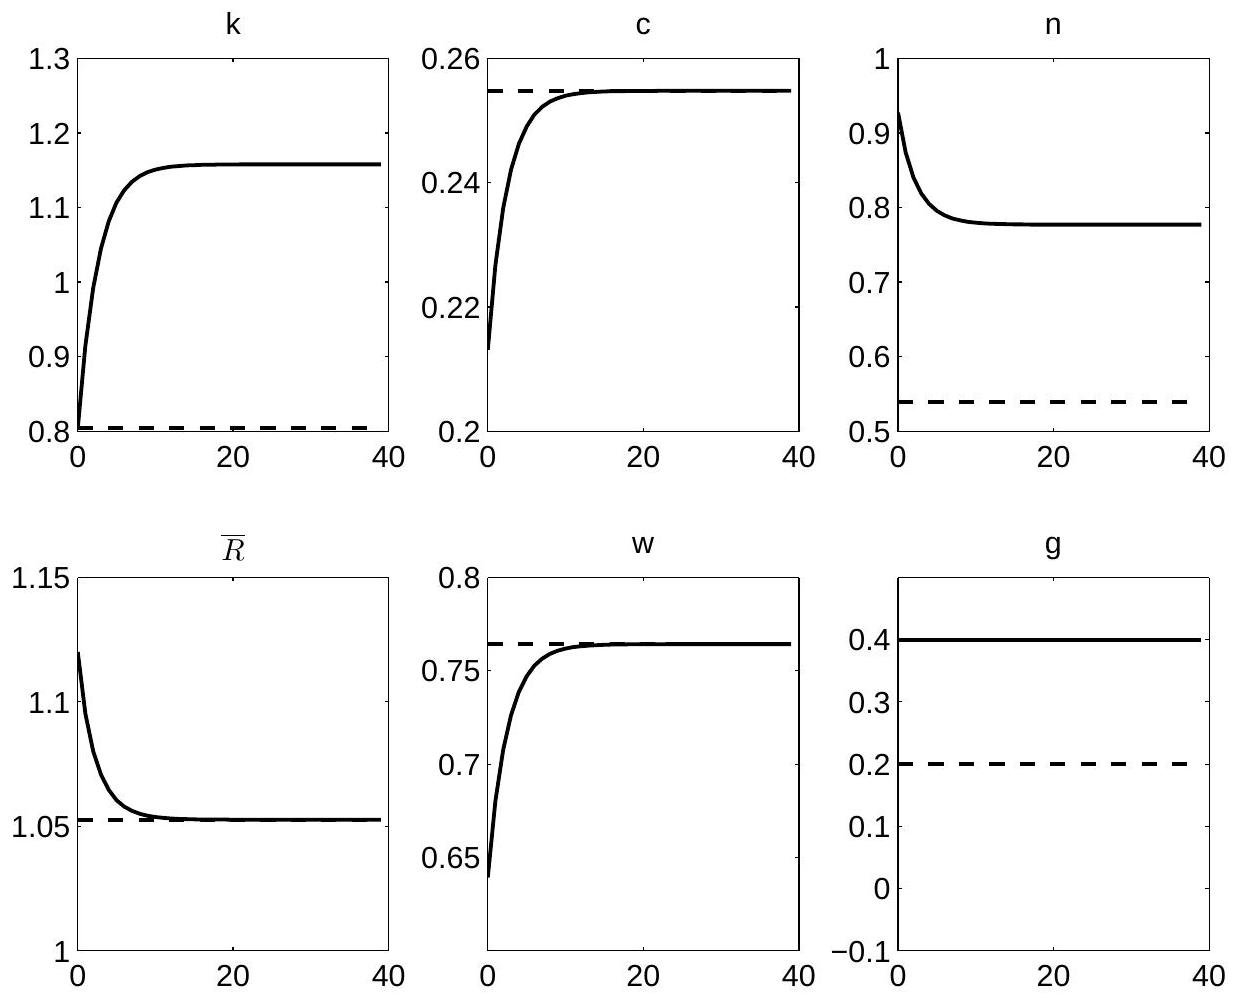
\includegraphics[width=\textwidth]{s05_04_01_g_legacy.jpg}
\captionsetup{labelformat=empty}
\caption{Figure 18: Elastic labor supply: response to unforeseen increase in g at $t=0$ (Figure 11.9.1).}
\end{center}
\label{fig:s05-04-01-g-legacy}
\end{figure}


\subsection*{5.4.2 Elastic Labor supply : Unforseen once-and-for-all increase in $\tau_{n}$ at $\mathbf{t}=\mathbf{0}$ (Figure 11.9.2).}
An unforeseen once-and-for-all increase in $\tau_{n}$ to 20 percentage points at $t=0$ (Figure 11.9.2).

\lstinputlisting{Code/sections/s05_04_02_taun.mod}

\begin{figure}[!htbp]
\begin{center}
  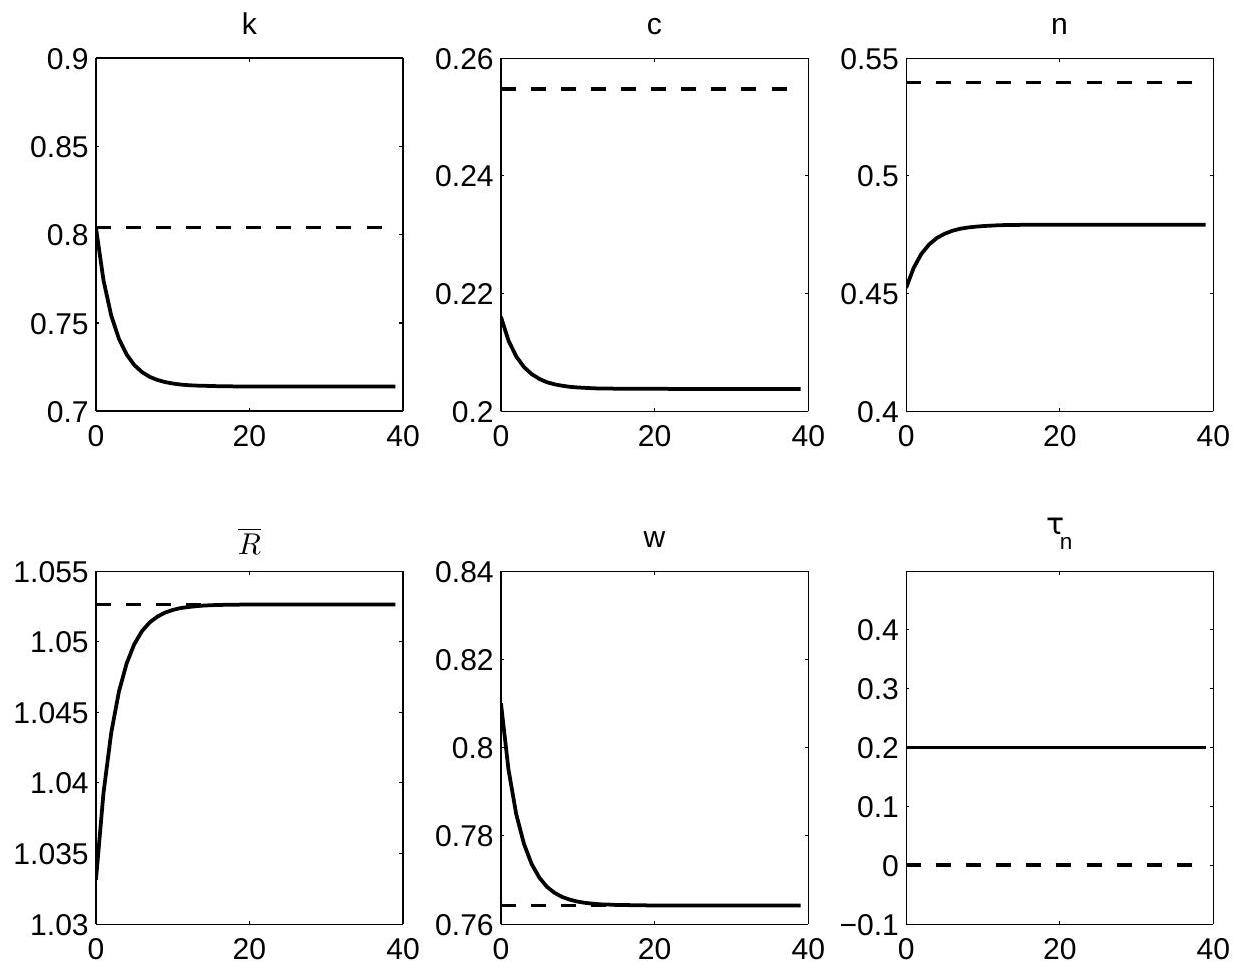
\includegraphics[width=\textwidth]{s05_04_02_taun_legacy.jpg}
\captionsetup{labelformat=empty}
\caption{Figure 19: Elastic labor supply: response to unforeseen increase in $\tau_n$ at $t=0$ (Figure 11.9.2).}
\end{center}
\label{fig:s05-04-02-taun-legacy}
\end{figure}


\subsection*{5.4.3 Elastic Labor supply : Foreseen once-and-for-all increase in $\tau_{n}$ at $\mathbf{t}=\mathbf{1 0}$ (Figure 11.9.3).}
A foreseen once-and-for-all increase in $\tau_{n}$ to 20 percentage points at $t=10$ (Figure 11.9.3).

\lstinputlisting{Code/sections/s05_04_03_taun.mod}

\begin{figure}[!htbp]
\begin{center}
  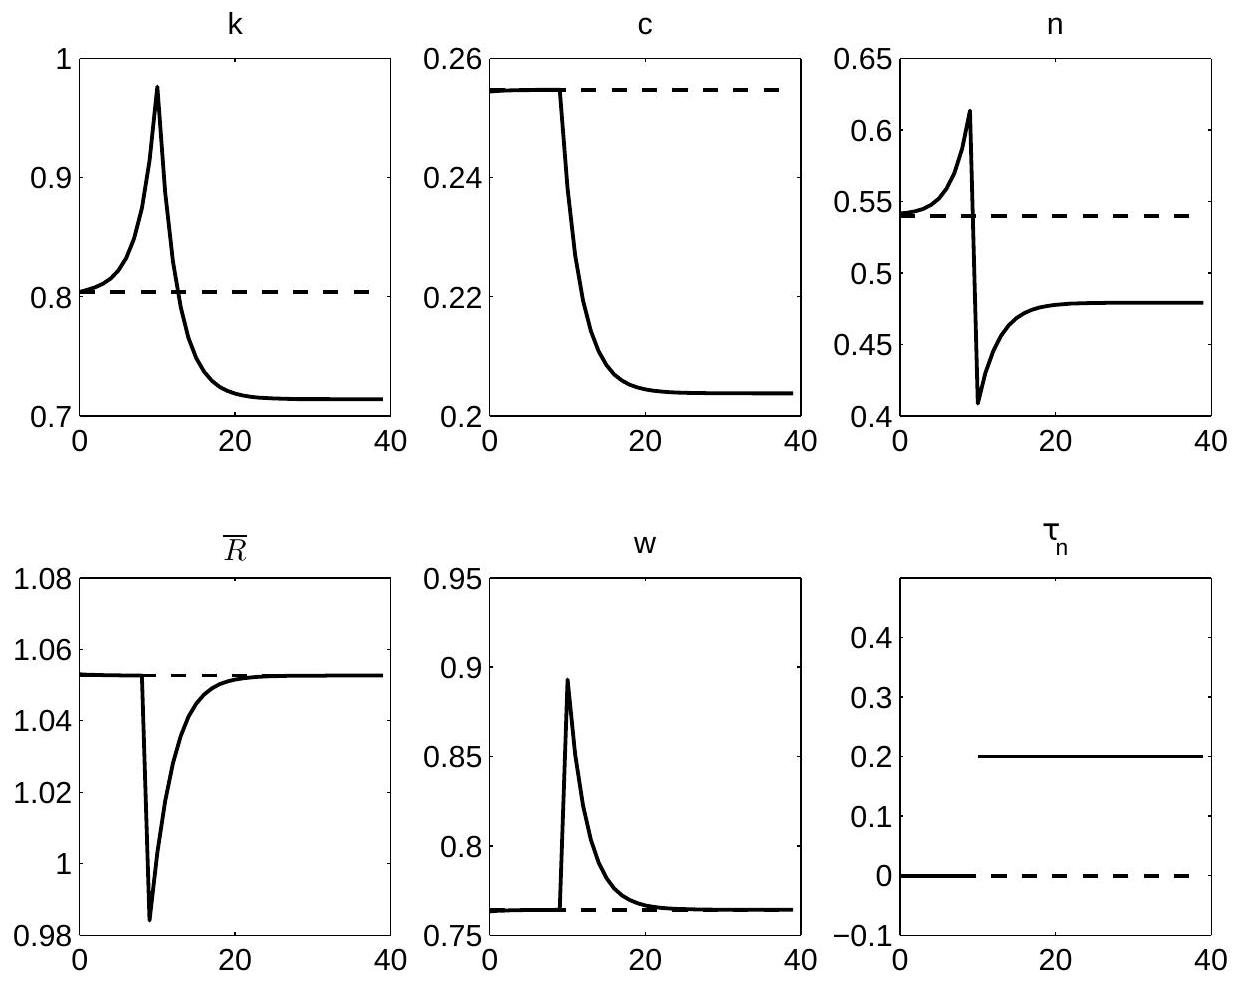
\includegraphics[width=\textwidth]{s05_04_03_taun_legacy.jpg}
\captionsetup{labelformat=empty}
\caption{Figure 20: Elastic labor supply: response to foreseen increase in $\tau_n$ at $t=10$ (Figure 11.9.3).}
\end{center}
\label{fig:s05-04-03-taun-legacy}
\end{figure}


\section{A full-scale fiscal RBC model}


This section is reserved for the flexible-price version of the separate NT-DSGE model. No verified implementation is included here; the archived generic RBC tax file must not be used as a substitute.


\appendix

\section*{A. List of Dynare Files}
The executable examples are in \texttt{Code/sections}. Run the approximation file before its corresponding estimation file to create the named simulated-data file. Section 4 files cover all six experiments; Section 5 files cover anticipated policies, both curvature calibrations, yield calculations, and three labour experiments. Section 6 has no verified local implementation. See \texttt{Code/README.md} for the inventory and run instructions and \texttt{review/REVIEW.md} for corrections and outstanding replication work.

\section*{References}
Cooley, T. F. and E. C. Prescott (1995). Economic growth and business cycles. In T. F. Cooley (Ed.), Frontiers of Business Cycle Research. Princeton University Press.

Kim, J. and S. H. Kim (2003, August). Spurious welfare reversals in international business cycle models. Journal of International Economics 60(2), 471-500.

Ljungqvist, L. and T. J. Sargent (2004). Recursive Macroeconomic Theory, Second edition. Cambridge, Ma.: MIT Press.

Ljungqvist, L. and T. J. Sargent (2012). Recursive Macroeconomic Theory, Third edition. Cambridge, Ma.: MIT Press.

Siow, A. (1984, May). Occupational choice under uncertainty. Econometrica 52(3), 631-45.


\end{document}